\documentclass[twoside]{book}

% Packages required by doxygen
\usepackage{calc}
\usepackage{doxygen}
\usepackage{graphicx}
\usepackage[utf8]{inputenc}
\usepackage{makeidx}
\usepackage{multicol}
\usepackage{multirow}
\usepackage{textcomp}
\usepackage[table]{xcolor}

% Font selection
\usepackage[T1]{fontenc}
\usepackage{mathptmx}
\usepackage[scaled=.90]{helvet}
\usepackage{courier}
\usepackage{amssymb}
\usepackage{sectsty}
\renewcommand{\familydefault}{\sfdefault}
\allsectionsfont{%
  \fontseries{bc}\selectfont%
  \color{darkgray}%
}
\renewcommand{\DoxyLabelFont}{%
  \fontseries{bc}\selectfont%
  \color{darkgray}%
}

% Page & text layout
\usepackage{geometry}
\geometry{%
  a4paper,%
  top=2.5cm,%
  bottom=2.5cm,%
  left=2.5cm,%
  right=2.5cm%
}
\tolerance=750
\hfuzz=15pt
\hbadness=750
\setlength{\emergencystretch}{15pt}
\setlength{\parindent}{0cm}
\setlength{\parskip}{0.2cm}
\makeatletter
\renewcommand{\paragraph}{%
  \@startsection{paragraph}{4}{0ex}{-1.0ex}{1.0ex}{%
    \normalfont\normalsize\bfseries\SS@parafont%
  }%
}
\renewcommand{\subparagraph}{%
  \@startsection{subparagraph}{5}{0ex}{-1.0ex}{1.0ex}{%
    \normalfont\normalsize\bfseries\SS@subparafont%
  }%
}
\makeatother

% Headers & footers
\usepackage{fancyhdr}
\pagestyle{fancyplain}
\fancyhead[LE]{\fancyplain{}{\bfseries\thepage}}
\fancyhead[CE]{\fancyplain{}{}}
\fancyhead[RE]{\fancyplain{}{\bfseries\leftmark}}
\fancyhead[LO]{\fancyplain{}{\bfseries\rightmark}}
\fancyhead[CO]{\fancyplain{}{}}
\fancyhead[RO]{\fancyplain{}{\bfseries\thepage}}
\fancyfoot[LE]{\fancyplain{}{}}
\fancyfoot[CE]{\fancyplain{}{}}
\fancyfoot[RE]{\fancyplain{}{\bfseries\scriptsize Generated on Tue Oct 29 2013 02\-:17\-:02 for sandbox by Doxygen }}
\fancyfoot[LO]{\fancyplain{}{\bfseries\scriptsize Generated on Tue Oct 29 2013 02\-:17\-:02 for sandbox by Doxygen }}
\fancyfoot[CO]{\fancyplain{}{}}
\fancyfoot[RO]{\fancyplain{}{}}
\renewcommand{\footrulewidth}{0.4pt}
\renewcommand{\chaptermark}[1]{%
  \markboth{#1}{}%
}
\renewcommand{\sectionmark}[1]{%
  \markright{\thesection\ #1}%
}

% Indices & bibliography
\usepackage{natbib}
\usepackage[titles]{tocloft}
\setcounter{tocdepth}{3}
\setcounter{secnumdepth}{5}
\makeindex

% Hyperlinks (required, but should be loaded last)
\usepackage{ifpdf}
\ifpdf
  \usepackage[pdftex,pagebackref=true]{hyperref}
\else
  \usepackage[ps2pdf,pagebackref=true]{hyperref}
\fi
\hypersetup{%
  colorlinks=true,%
  linkcolor=blue,%
  citecolor=blue,%
  unicode%
}

% Custom commands
\newcommand{\clearemptydoublepage}{%
  \newpage{\pagestyle{empty}\cleardoublepage}%
}


%===== C O N T E N T S =====

\begin{document}

% Titlepage & ToC
\hypersetup{pageanchor=false}
\pagenumbering{roman}
\begin{titlepage}
\vspace*{7cm}
\begin{center}%
{\Large sandbox }\\
\vspace*{1cm}
{\large Generated by Doxygen 1.8.5}\\
\vspace*{0.5cm}
{\small Tue Oct 29 2013 02:17:02}\\
\end{center}
\end{titlepage}
\clearemptydoublepage
\tableofcontents
\clearemptydoublepage
\pagenumbering{arabic}
\hypersetup{pageanchor=true}

%--- Begin generated contents ---
\chapter{Namespace Index}
\section{Namespace List}
Here is a list of all namespaces with brief descriptions\-:\begin{DoxyCompactList}
\item\contentsline{section}{\hyperlink{namespacesandbox}{sandbox} }{\pageref{namespacesandbox}}{}
\item\contentsline{section}{\hyperlink{namespacesandbox_1_1pattern}{sandbox\-::pattern} }{\pageref{namespacesandbox_1_1pattern}}{}
\end{DoxyCompactList}

\chapter{Hierarchical Index}
\section{Class Hierarchy}
This inheritance list is sorted roughly, but not completely, alphabetically\-:\begin{DoxyCompactList}
\item \contentsline{section}{Abstract\-Algorithm}{\pageref{class_abstract_algorithm}}{}
\begin{DoxyCompactList}
\item \contentsline{section}{Concrete\-Algorithm}{\pageref{class_concrete_algorithm}}{}
\end{DoxyCompactList}
\item \contentsline{section}{sandbox\-:\-:Options}{\pageref{classsandbox_1_1_options}}{}
\item \contentsline{section}{sandbox\-:\-:pattern\-:\-:Singleton}{\pageref{classsandbox_1_1pattern_1_1_singleton}}{}
\item \contentsline{section}{sandbox\-:\-:Time\-Type}{\pageref{classsandbox_1_1_time_type}}{}
\item \contentsline{section}{sandbox\-:\-:pattern\-:\-:Tool}{\pageref{classsandbox_1_1pattern_1_1_tool}}{}
\begin{DoxyCompactList}
\item \contentsline{section}{sandbox\-:\-:pattern\-:\-:Draw\-Tool}{\pageref{classsandbox_1_1pattern_1_1_draw_tool}}{}
\item \contentsline{section}{sandbox\-:\-:pattern\-:\-:State\-Select}{\pageref{classsandbox_1_1pattern_1_1_state_select}}{}
\end{DoxyCompactList}
\item \contentsline{section}{sandbox\-:\-:pattern\-:\-:Tool\-Controller}{\pageref{classsandbox_1_1pattern_1_1_tool_controller}}{}
\item \contentsline{section}{sandbox\-:\-:Variant}{\pageref{classsandbox_1_1_variant}}{}
\end{DoxyCompactList}

\chapter{Class Index}
\section{Class List}
Here are the classes, structs, unions and interfaces with brief descriptions\-:\begin{DoxyCompactList}
\item\contentsline{section}{\hyperlink{class_abstract_algorithm}{Abstract\-Algorithm} }{\pageref{class_abstract_algorithm}}{}
\item\contentsline{section}{\hyperlink{class_concrete_algorithm}{Concrete\-Algorithm} }{\pageref{class_concrete_algorithm}}{}
\item\contentsline{section}{\hyperlink{classsandbox_1_1pattern_1_1_draw_tool}{sandbox\-::pattern\-::\-Draw\-Tool} }{\pageref{classsandbox_1_1pattern_1_1_draw_tool}}{}
\item\contentsline{section}{\hyperlink{classsandbox_1_1_options}{sandbox\-::\-Options} }{\pageref{classsandbox_1_1_options}}{}
\item\contentsline{section}{\hyperlink{classsandbox_1_1pattern_1_1_singleton}{sandbox\-::pattern\-::\-Singleton} }{\pageref{classsandbox_1_1pattern_1_1_singleton}}{}
\item\contentsline{section}{\hyperlink{classsandbox_1_1pattern_1_1_state_select}{sandbox\-::pattern\-::\-State\-Select} }{\pageref{classsandbox_1_1pattern_1_1_state_select}}{}
\item\contentsline{section}{\hyperlink{classsandbox_1_1_time_type}{sandbox\-::\-Time\-Type} }{\pageref{classsandbox_1_1_time_type}}{}
\item\contentsline{section}{\hyperlink{classsandbox_1_1pattern_1_1_tool}{sandbox\-::pattern\-::\-Tool} }{\pageref{classsandbox_1_1pattern_1_1_tool}}{}
\item\contentsline{section}{\hyperlink{classsandbox_1_1pattern_1_1_tool_controller}{sandbox\-::pattern\-::\-Tool\-Controller} }{\pageref{classsandbox_1_1pattern_1_1_tool_controller}}{}
\item\contentsline{section}{\hyperlink{classsandbox_1_1_variant}{sandbox\-::\-Variant} }{\pageref{classsandbox_1_1_variant}}{}
\end{DoxyCompactList}

\chapter{File Index}
\section{File List}
Here is a list of all files with brief descriptions\-:\begin{DoxyCompactList}
\item\contentsline{section}{F\-:/\-Projects/sandbox/src/\hyperlink{main_8cpp}{main.\-cpp} }{\pageref{main_8cpp}}{}
\item\contentsline{section}{F\-:/\-Projects/sandbox/src/\hyperlink{options_8h}{options.\-h} }{\pageref{options_8h}}{}
\item\contentsline{section}{F\-:/\-Projects/sandbox/src/\hyperlink{quicksort_8h}{quicksort.\-h} }{\pageref{quicksort_8h}}{}
\item\contentsline{section}{F\-:/\-Projects/sandbox/src/\hyperlink{shed_8h}{shed.\-h} }{\pageref{shed_8h}}{}
\item\contentsline{section}{F\-:/\-Projects/sandbox/src/\hyperlink{timetype_8cpp}{timetype.\-cpp} }{\pageref{timetype_8cpp}}{}
\item\contentsline{section}{F\-:/\-Projects/sandbox/src/\hyperlink{timetype_8h}{timetype.\-h} }{\pageref{timetype_8h}}{}
\item\contentsline{section}{F\-:/\-Projects/sandbox/src/\hyperlink{variant_8h}{variant.\-h} }{\pageref{variant_8h}}{}
\item\contentsline{section}{F\-:/\-Projects/sandbox/src/boost/\hyperlink{chromaaberration_8cpp}{chromaaberration.\-cpp} }{\pageref{chromaaberration_8cpp}}{}
\item\contentsline{section}{F\-:/\-Projects/sandbox/src/boost/\hyperlink{chromaaberration_8h}{chromaaberration.\-h} }{\pageref{chromaaberration_8h}}{}
\item\contentsline{section}{F\-:/\-Projects/sandbox/src/pattern/\hyperlink{singleton_8h}{singleton.\-h} }{\pageref{singleton_8h}}{}
\item\contentsline{section}{F\-:/\-Projects/sandbox/src/pattern/\hyperlink{state_8h}{state.\-h} }{\pageref{state_8h}}{}
\item\contentsline{section}{F\-:/\-Projects/sandbox/src/pattern/\hyperlink{strategy_8h}{strategy.\-h} }{\pageref{strategy_8h}}{}
\item\contentsline{section}{F\-:/\-Projects/sandbox/src/pattern/\hyperlink{template_method_8h}{template\-Method.\-h} }{\pageref{template_method_8h}}{}
\end{DoxyCompactList}

\chapter{Namespace Documentation}
\hypertarget{namespacesandbox}{\section{sandbox Namespace Reference}
\label{namespacesandbox}\index{sandbox@{sandbox}}
}
\subsection*{Namespaces}
\begin{DoxyCompactItemize}
\item 
\hyperlink{namespacesandbox_1_1pattern}{pattern}
\end{DoxyCompactItemize}
\subsection*{Classes}
\begin{DoxyCompactItemize}
\item 
class \hyperlink{classsandbox_1_1_options}{Options}
\item 
class \hyperlink{classsandbox_1_1_time_type}{Time\-Type}
\item 
class \hyperlink{classsandbox_1_1_variant}{Variant}
\end{DoxyCompactItemize}
\subsection*{Functions}
\begin{DoxyCompactItemize}
\item 
std\-::ostream \& \hyperlink{namespacesandbox_a8ca45cec79e562a7f2322662d281d1b4}{operator$<$$<$} (std\-::ostream \&output, \hyperlink{classsandbox_1_1_options}{Options} \&options)
\begin{DoxyCompactList}\small\item\em Writes all data to a output stream. \end{DoxyCompactList}\item 
std\-::istream \& \hyperlink{namespacesandbox_ab63c581d554f481ae6d06c434db5f7e5}{operator$>$$>$} (std\-::istream \&input, \hyperlink{classsandbox_1_1_options}{Options} \&options)
\begin{DoxyCompactList}\small\item\em Reads key value pairs from an input stream. it's throws Options\-::invalid\-\_\-format exception on misformatted input. \end{DoxyCompactList}\item 
{\footnotesize template$<$typename Iterator $>$ }\\void \hyperlink{namespacesandbox_a9f8d9538b5bfad2fd243b182598f994e}{print\-Out} (Iterator front, Iterator back)
\item 
{\footnotesize template$<$typename Iterator $>$ }\\void \hyperlink{namespacesandbox_a7d82a406c267d30ff1f27c5ff300437a}{quick\-Sort} (Iterator front, Iterator back)
\item 
{\footnotesize template$<$typename T $>$ }\\std\-::vector$<$ T $>$ \& \hyperlink{namespacesandbox_a85c255856530c2a1f629abb6bf2f4497}{quick\-Sort} (std\-::vector$<$ T $>$ \&sortable)
\item 
{\footnotesize template$<$typename Iterator $>$ }\\bool \hyperlink{namespacesandbox_a25a11dad06fc0cd1b3f9bc583f093636}{is\-Palindrome} (Iterator front, Iterator back)
\item 
bool \hyperlink{namespacesandbox_a4a569da66e67b46889d0c0597b7196b0}{is\-Palindrome} (std\-::string const \&str)
\item 
bool \hyperlink{namespacesandbox_a639859e1234594e142ea447fad2b3b34}{is\-Palindrome} (char const $\ast$str)
\item 
bool \hyperlink{namespacesandbox_a563b930dc7888d8ab257fe747fa53487}{is\-Little\-Endian} ()
\item 
bool \hyperlink{namespacesandbox_a550f00cb3d4e2ac434c7b76532e79573}{is\-Big\-Endian} ()
\item 
{\footnotesize template$<$typename T $>$ }\\void \hyperlink{namespacesandbox_a78a289ddc885bdcb5383f1363c54db2c}{swap} (T \&a, T \&b)
\item 
{\footnotesize template$<$typename Iterator $>$ }\\void \hyperlink{namespacesandbox_af7dc9a62c4e56b2b4c4a12ff6e82a237}{swap\-In\-Range} (Iterator front, Iterator back)
\item 
std\-::string \& \hyperlink{namespacesandbox_acb1d210d07ad7665578cbcb47c995332}{reverse} (std\-::string \&str)
\item 
char $\ast$ \hyperlink{namespacesandbox_a71d57df2b65e2db22f1b6126cf5305ec}{reverse} (char $\ast$str)
\item 
std\-::string \& \hyperlink{namespacesandbox_aa4f703c0251f20815a2f7d99bf55b9a8}{reverse\-Words} (std\-::string \&str)
\item 
std\-::ostream \& \hyperlink{namespacesandbox_a1d6485022eb73d061719402a29c67183}{operator$<$$<$} (std\-::ostream \&output, \hyperlink{classsandbox_1_1_variant}{Variant} const \&variant)
\end{DoxyCompactItemize}


\subsection{Function Documentation}
\hypertarget{namespacesandbox_a550f00cb3d4e2ac434c7b76532e79573}{\index{sandbox@{sandbox}!is\-Big\-Endian@{is\-Big\-Endian}}
\index{is\-Big\-Endian@{is\-Big\-Endian}!sandbox@{sandbox}}
\subsubsection[{is\-Big\-Endian}]{\setlength{\rightskip}{0pt plus 5cm}bool sandbox\-::is\-Big\-Endian (
\begin{DoxyParamCaption}
{}
\end{DoxyParamCaption}
)\hspace{0.3cm}{\ttfamily [inline]}}}\label{namespacesandbox_a550f00cb3d4e2ac434c7b76532e79573}
\hypertarget{namespacesandbox_a563b930dc7888d8ab257fe747fa53487}{\index{sandbox@{sandbox}!is\-Little\-Endian@{is\-Little\-Endian}}
\index{is\-Little\-Endian@{is\-Little\-Endian}!sandbox@{sandbox}}
\subsubsection[{is\-Little\-Endian}]{\setlength{\rightskip}{0pt plus 5cm}bool sandbox\-::is\-Little\-Endian (
\begin{DoxyParamCaption}
{}
\end{DoxyParamCaption}
)\hspace{0.3cm}{\ttfamily [inline]}}}\label{namespacesandbox_a563b930dc7888d8ab257fe747fa53487}
\hypertarget{namespacesandbox_a25a11dad06fc0cd1b3f9bc583f093636}{\index{sandbox@{sandbox}!is\-Palindrome@{is\-Palindrome}}
\index{is\-Palindrome@{is\-Palindrome}!sandbox@{sandbox}}
\subsubsection[{is\-Palindrome}]{\setlength{\rightskip}{0pt plus 5cm}template$<$typename Iterator $>$ bool sandbox\-::is\-Palindrome (
\begin{DoxyParamCaption}
\item[{Iterator}]{front, }
\item[{Iterator}]{back}
\end{DoxyParamCaption}
)\hspace{0.3cm}{\ttfamily [inline]}}}\label{namespacesandbox_a25a11dad06fc0cd1b3f9bc583f093636}
\hypertarget{namespacesandbox_a4a569da66e67b46889d0c0597b7196b0}{\index{sandbox@{sandbox}!is\-Palindrome@{is\-Palindrome}}
\index{is\-Palindrome@{is\-Palindrome}!sandbox@{sandbox}}
\subsubsection[{is\-Palindrome}]{\setlength{\rightskip}{0pt plus 5cm}bool sandbox\-::is\-Palindrome (
\begin{DoxyParamCaption}
\item[{std\-::string const \&}]{str}
\end{DoxyParamCaption}
)\hspace{0.3cm}{\ttfamily [inline]}}}\label{namespacesandbox_a4a569da66e67b46889d0c0597b7196b0}
\hypertarget{namespacesandbox_a639859e1234594e142ea447fad2b3b34}{\index{sandbox@{sandbox}!is\-Palindrome@{is\-Palindrome}}
\index{is\-Palindrome@{is\-Palindrome}!sandbox@{sandbox}}
\subsubsection[{is\-Palindrome}]{\setlength{\rightskip}{0pt plus 5cm}bool sandbox\-::is\-Palindrome (
\begin{DoxyParamCaption}
\item[{char const $\ast$}]{str}
\end{DoxyParamCaption}
)\hspace{0.3cm}{\ttfamily [inline]}}}\label{namespacesandbox_a639859e1234594e142ea447fad2b3b34}
\hypertarget{namespacesandbox_a8ca45cec79e562a7f2322662d281d1b4}{\index{sandbox@{sandbox}!operator$<$$<$@{operator$<$$<$}}
\index{operator$<$$<$@{operator$<$$<$}!sandbox@{sandbox}}
\subsubsection[{operator$<$$<$}]{\setlength{\rightskip}{0pt plus 5cm}std\-::ostream\& sandbox\-::operator$<$$<$ (
\begin{DoxyParamCaption}
\item[{std\-::ostream \&}]{output, }
\item[{Options \&}]{options}
\end{DoxyParamCaption}
)\hspace{0.3cm}{\ttfamily [inline]}}}\label{namespacesandbox_a8ca45cec79e562a7f2322662d281d1b4}


Writes all data to a output stream. 

\hypertarget{namespacesandbox_a1d6485022eb73d061719402a29c67183}{\index{sandbox@{sandbox}!operator$<$$<$@{operator$<$$<$}}
\index{operator$<$$<$@{operator$<$$<$}!sandbox@{sandbox}}
\subsubsection[{operator$<$$<$}]{\setlength{\rightskip}{0pt plus 5cm}std\-::ostream\& sandbox\-::operator$<$$<$ (
\begin{DoxyParamCaption}
\item[{std\-::ostream \&}]{output, }
\item[{Variant const \&}]{variant}
\end{DoxyParamCaption}
)\hspace{0.3cm}{\ttfamily [inline]}}}\label{namespacesandbox_a1d6485022eb73d061719402a29c67183}
\hypertarget{namespacesandbox_ab63c581d554f481ae6d06c434db5f7e5}{\index{sandbox@{sandbox}!operator$>$$>$@{operator$>$$>$}}
\index{operator$>$$>$@{operator$>$$>$}!sandbox@{sandbox}}
\subsubsection[{operator$>$$>$}]{\setlength{\rightskip}{0pt plus 5cm}std\-::istream\& sandbox\-::operator$>$$>$ (
\begin{DoxyParamCaption}
\item[{std\-::istream \&}]{input, }
\item[{Options \&}]{options}
\end{DoxyParamCaption}
)\hspace{0.3cm}{\ttfamily [inline]}}}\label{namespacesandbox_ab63c581d554f481ae6d06c434db5f7e5}


Reads key value pairs from an input stream. it's throws Options\-::invalid\-\_\-format exception on misformatted input. 

\hypertarget{namespacesandbox_a9f8d9538b5bfad2fd243b182598f994e}{\index{sandbox@{sandbox}!print\-Out@{print\-Out}}
\index{print\-Out@{print\-Out}!sandbox@{sandbox}}
\subsubsection[{print\-Out}]{\setlength{\rightskip}{0pt plus 5cm}template$<$typename Iterator $>$ void sandbox\-::print\-Out (
\begin{DoxyParamCaption}
\item[{Iterator}]{front, }
\item[{Iterator}]{back}
\end{DoxyParamCaption}
)\hspace{0.3cm}{\ttfamily [inline]}}}\label{namespacesandbox_a9f8d9538b5bfad2fd243b182598f994e}
\hypertarget{namespacesandbox_a7d82a406c267d30ff1f27c5ff300437a}{\index{sandbox@{sandbox}!quick\-Sort@{quick\-Sort}}
\index{quick\-Sort@{quick\-Sort}!sandbox@{sandbox}}
\subsubsection[{quick\-Sort}]{\setlength{\rightskip}{0pt plus 5cm}template$<$typename Iterator $>$ void sandbox\-::quick\-Sort (
\begin{DoxyParamCaption}
\item[{Iterator}]{front, }
\item[{Iterator}]{back}
\end{DoxyParamCaption}
)\hspace{0.3cm}{\ttfamily [inline]}}}\label{namespacesandbox_a7d82a406c267d30ff1f27c5ff300437a}
\hypertarget{namespacesandbox_a85c255856530c2a1f629abb6bf2f4497}{\index{sandbox@{sandbox}!quick\-Sort@{quick\-Sort}}
\index{quick\-Sort@{quick\-Sort}!sandbox@{sandbox}}
\subsubsection[{quick\-Sort}]{\setlength{\rightskip}{0pt plus 5cm}template$<$typename T $>$ std\-::vector$<$T$>$\& sandbox\-::quick\-Sort (
\begin{DoxyParamCaption}
\item[{std\-::vector$<$ T $>$ \&}]{sortable}
\end{DoxyParamCaption}
)\hspace{0.3cm}{\ttfamily [inline]}}}\label{namespacesandbox_a85c255856530c2a1f629abb6bf2f4497}
\hypertarget{namespacesandbox_acb1d210d07ad7665578cbcb47c995332}{\index{sandbox@{sandbox}!reverse@{reverse}}
\index{reverse@{reverse}!sandbox@{sandbox}}
\subsubsection[{reverse}]{\setlength{\rightskip}{0pt plus 5cm}std\-::string\& sandbox\-::reverse (
\begin{DoxyParamCaption}
\item[{std\-::string \&}]{str}
\end{DoxyParamCaption}
)\hspace{0.3cm}{\ttfamily [inline]}}}\label{namespacesandbox_acb1d210d07ad7665578cbcb47c995332}
\hypertarget{namespacesandbox_a71d57df2b65e2db22f1b6126cf5305ec}{\index{sandbox@{sandbox}!reverse@{reverse}}
\index{reverse@{reverse}!sandbox@{sandbox}}
\subsubsection[{reverse}]{\setlength{\rightskip}{0pt plus 5cm}char$\ast$ sandbox\-::reverse (
\begin{DoxyParamCaption}
\item[{char $\ast$}]{str}
\end{DoxyParamCaption}
)\hspace{0.3cm}{\ttfamily [inline]}}}\label{namespacesandbox_a71d57df2b65e2db22f1b6126cf5305ec}
\hypertarget{namespacesandbox_aa4f703c0251f20815a2f7d99bf55b9a8}{\index{sandbox@{sandbox}!reverse\-Words@{reverse\-Words}}
\index{reverse\-Words@{reverse\-Words}!sandbox@{sandbox}}
\subsubsection[{reverse\-Words}]{\setlength{\rightskip}{0pt plus 5cm}std\-::string\& sandbox\-::reverse\-Words (
\begin{DoxyParamCaption}
\item[{std\-::string \&}]{str}
\end{DoxyParamCaption}
)\hspace{0.3cm}{\ttfamily [inline]}}}\label{namespacesandbox_aa4f703c0251f20815a2f7d99bf55b9a8}
\hypertarget{namespacesandbox_a78a289ddc885bdcb5383f1363c54db2c}{\index{sandbox@{sandbox}!swap@{swap}}
\index{swap@{swap}!sandbox@{sandbox}}
\subsubsection[{swap}]{\setlength{\rightskip}{0pt plus 5cm}template$<$typename T $>$ void sandbox\-::swap (
\begin{DoxyParamCaption}
\item[{T \&}]{a, }
\item[{T \&}]{b}
\end{DoxyParamCaption}
)\hspace{0.3cm}{\ttfamily [inline]}}}\label{namespacesandbox_a78a289ddc885bdcb5383f1363c54db2c}
\hypertarget{namespacesandbox_af7dc9a62c4e56b2b4c4a12ff6e82a237}{\index{sandbox@{sandbox}!swap\-In\-Range@{swap\-In\-Range}}
\index{swap\-In\-Range@{swap\-In\-Range}!sandbox@{sandbox}}
\subsubsection[{swap\-In\-Range}]{\setlength{\rightskip}{0pt plus 5cm}template$<$typename Iterator $>$ void sandbox\-::swap\-In\-Range (
\begin{DoxyParamCaption}
\item[{Iterator}]{front, }
\item[{Iterator}]{back}
\end{DoxyParamCaption}
)\hspace{0.3cm}{\ttfamily [inline]}}}\label{namespacesandbox_af7dc9a62c4e56b2b4c4a12ff6e82a237}

\hypertarget{namespacesandbox_1_1pattern}{\section{sandbox\-:\-:pattern Namespace Reference}
\label{namespacesandbox_1_1pattern}\index{sandbox\-::pattern@{sandbox\-::pattern}}
}
\subsection*{Classes}
\begin{DoxyCompactItemize}
\item 
class \hyperlink{classsandbox_1_1pattern_1_1_singleton}{Singleton}
\item 
class \hyperlink{classsandbox_1_1pattern_1_1_tool}{Tool}
\item 
class \hyperlink{classsandbox_1_1pattern_1_1_draw_tool}{Draw\-Tool}
\item 
class \hyperlink{classsandbox_1_1pattern_1_1_state_select}{State\-Select}
\item 
class \hyperlink{classsandbox_1_1pattern_1_1_tool_controller}{Tool\-Controller}
\end{DoxyCompactItemize}

\chapter{Class Documentation}
\hypertarget{class_abstract_algorithm}{\section{Abstract\-Algorithm Class Reference}
\label{class_abstract_algorithm}\index{Abstract\-Algorithm@{Abstract\-Algorithm}}
}


{\ttfamily \#include $<$template\-Method.\-h$>$}

Inheritance diagram for Abstract\-Algorithm\-:\begin{figure}[H]
\begin{center}
\leavevmode
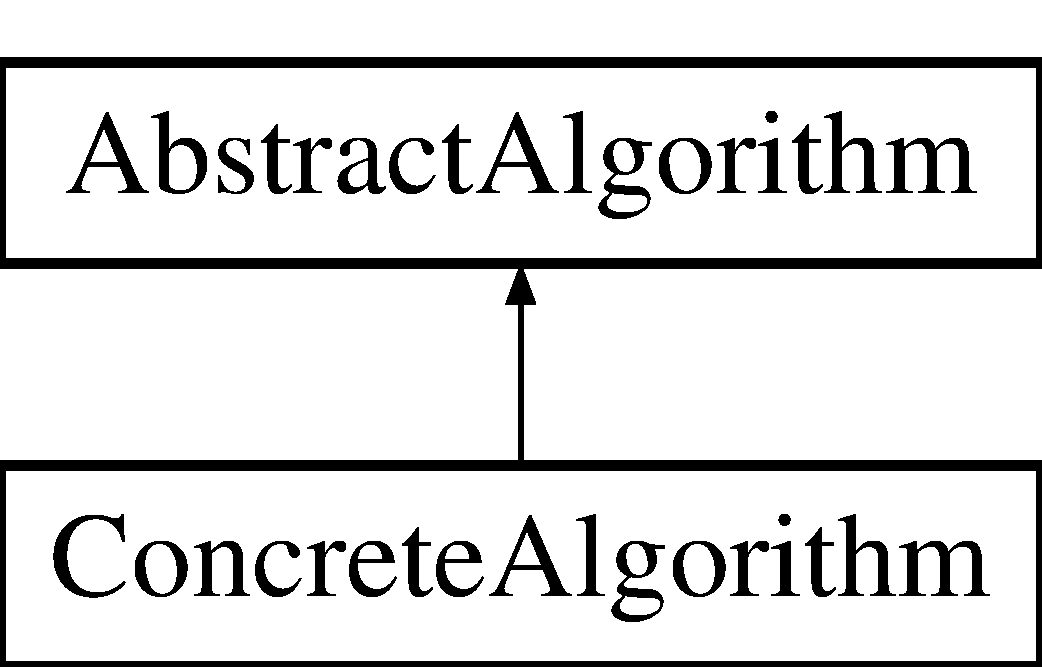
\includegraphics[height=2.000000cm]{class_abstract_algorithm}
\end{center}
\end{figure}
\subsection*{Public Member Functions}
\begin{DoxyCompactItemize}
\item 
void \hyperlink{class_abstract_algorithm_a7d8715fc465cc79c1131832989fbdf82}{operation} ()
\end{DoxyCompactItemize}
\subsection*{Protected Member Functions}
\begin{DoxyCompactItemize}
\item 
virtual void \hyperlink{class_abstract_algorithm_a860e4d98800f4dceb5721d835d5ceeb0}{do\-Operation1} ()=0
\item 
virtual void \hyperlink{class_abstract_algorithm_ae758fdd33b4bd3ba12c9d49ce6fad741}{do\-Operation2} ()=0
\item 
virtual void \hyperlink{class_abstract_algorithm_abef35c1f2097de614a14c2daa24b16c5}{do\-Operation3} ()=0
\end{DoxyCompactItemize}


\subsection{Member Function Documentation}
\hypertarget{class_abstract_algorithm_a860e4d98800f4dceb5721d835d5ceeb0}{\index{Abstract\-Algorithm@{Abstract\-Algorithm}!do\-Operation1@{do\-Operation1}}
\index{do\-Operation1@{do\-Operation1}!AbstractAlgorithm@{Abstract\-Algorithm}}
\subsubsection[{do\-Operation1}]{\setlength{\rightskip}{0pt plus 5cm}virtual void Abstract\-Algorithm\-::do\-Operation1 (
\begin{DoxyParamCaption}
{}
\end{DoxyParamCaption}
)\hspace{0.3cm}{\ttfamily [protected]}, {\ttfamily [pure virtual]}}}\label{class_abstract_algorithm_a860e4d98800f4dceb5721d835d5ceeb0}
\hypertarget{class_abstract_algorithm_ae758fdd33b4bd3ba12c9d49ce6fad741}{\index{Abstract\-Algorithm@{Abstract\-Algorithm}!do\-Operation2@{do\-Operation2}}
\index{do\-Operation2@{do\-Operation2}!AbstractAlgorithm@{Abstract\-Algorithm}}
\subsubsection[{do\-Operation2}]{\setlength{\rightskip}{0pt plus 5cm}virtual void Abstract\-Algorithm\-::do\-Operation2 (
\begin{DoxyParamCaption}
{}
\end{DoxyParamCaption}
)\hspace{0.3cm}{\ttfamily [protected]}, {\ttfamily [pure virtual]}}}\label{class_abstract_algorithm_ae758fdd33b4bd3ba12c9d49ce6fad741}
\hypertarget{class_abstract_algorithm_abef35c1f2097de614a14c2daa24b16c5}{\index{Abstract\-Algorithm@{Abstract\-Algorithm}!do\-Operation3@{do\-Operation3}}
\index{do\-Operation3@{do\-Operation3}!AbstractAlgorithm@{Abstract\-Algorithm}}
\subsubsection[{do\-Operation3}]{\setlength{\rightskip}{0pt plus 5cm}virtual void Abstract\-Algorithm\-::do\-Operation3 (
\begin{DoxyParamCaption}
{}
\end{DoxyParamCaption}
)\hspace{0.3cm}{\ttfamily [protected]}, {\ttfamily [pure virtual]}}}\label{class_abstract_algorithm_abef35c1f2097de614a14c2daa24b16c5}
\hypertarget{class_abstract_algorithm_a7d8715fc465cc79c1131832989fbdf82}{\index{Abstract\-Algorithm@{Abstract\-Algorithm}!operation@{operation}}
\index{operation@{operation}!AbstractAlgorithm@{Abstract\-Algorithm}}
\subsubsection[{operation}]{\setlength{\rightskip}{0pt plus 5cm}void Abstract\-Algorithm\-::operation (
\begin{DoxyParamCaption}
{}
\end{DoxyParamCaption}
)\hspace{0.3cm}{\ttfamily [inline]}}}\label{class_abstract_algorithm_a7d8715fc465cc79c1131832989fbdf82}


The documentation for this class was generated from the following file\-:\begin{DoxyCompactItemize}
\item 
F\-:/\-Projects/sandbox/src/pattern/\hyperlink{template_method_8h}{template\-Method.\-h}\end{DoxyCompactItemize}

\hypertarget{class_concrete_algorithm}{\section{Concrete\-Algorithm Class Reference}
\label{class_concrete_algorithm}\index{Concrete\-Algorithm@{Concrete\-Algorithm}}
}


{\ttfamily \#include $<$template\-Method.\-h$>$}

Inheritance diagram for Concrete\-Algorithm\-:\begin{figure}[H]
\begin{center}
\leavevmode
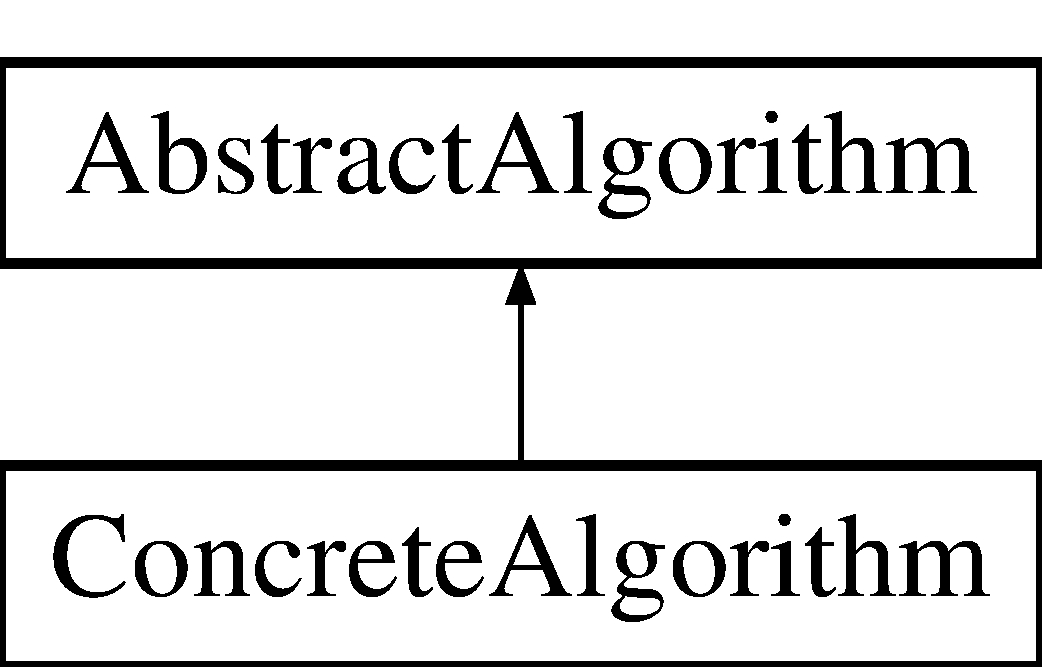
\includegraphics[height=2.000000cm]{class_concrete_algorithm}
\end{center}
\end{figure}
\subsection*{Additional Inherited Members}


The documentation for this class was generated from the following file\-:\begin{DoxyCompactItemize}
\item 
F\-:/\-Projects/sandbox/src/pattern/\hyperlink{template_method_8h}{template\-Method.\-h}\end{DoxyCompactItemize}

\hypertarget{classsandbox_1_1pattern_1_1_draw_tool}{\section{sandbox\-:\-:pattern\-:\-:Draw\-Tool Class Reference}
\label{classsandbox_1_1pattern_1_1_draw_tool}\index{sandbox\-::pattern\-::\-Draw\-Tool@{sandbox\-::pattern\-::\-Draw\-Tool}}
}


{\ttfamily \#include $<$state.\-h$>$}

Inheritance diagram for sandbox\-:\-:pattern\-:\-:Draw\-Tool\-:\begin{figure}[H]
\begin{center}
\leavevmode
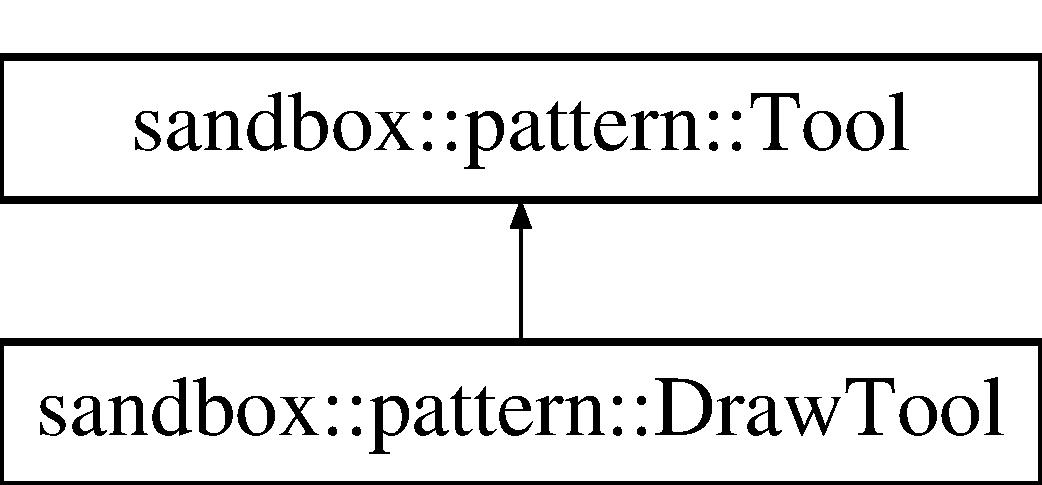
\includegraphics[height=2.000000cm]{classsandbox_1_1pattern_1_1_draw_tool}
\end{center}
\end{figure}
\subsection*{Public Member Functions}
\begin{DoxyCompactItemize}
\item 
void \hyperlink{classsandbox_1_1pattern_1_1_draw_tool_af43b828fa933c2ee66279f378cda067d}{on\-Mouse\-Down} (\hyperlink{classsandbox_1_1pattern_1_1_tool_controller}{Tool\-Controller} $\ast$controller)
\item 
void \hyperlink{classsandbox_1_1pattern_1_1_draw_tool_a3cb662ec466497fdfc9b69b2a4b1fcdb}{on\-Mouse\-Up} (\hyperlink{classsandbox_1_1pattern_1_1_tool_controller}{Tool\-Controller} $\ast$controller)
\item 
void \hyperlink{classsandbox_1_1pattern_1_1_draw_tool_a66e92b8b6ca5b9623203051bb31151bf}{on\-Mouse\-Move} (\hyperlink{classsandbox_1_1pattern_1_1_tool_controller}{Tool\-Controller} $\ast$controller)
\end{DoxyCompactItemize}


\subsection{Member Function Documentation}
\hypertarget{classsandbox_1_1pattern_1_1_draw_tool_af43b828fa933c2ee66279f378cda067d}{\index{sandbox\-::pattern\-::\-Draw\-Tool@{sandbox\-::pattern\-::\-Draw\-Tool}!on\-Mouse\-Down@{on\-Mouse\-Down}}
\index{on\-Mouse\-Down@{on\-Mouse\-Down}!sandbox::pattern::DrawTool@{sandbox\-::pattern\-::\-Draw\-Tool}}
\subsubsection[{on\-Mouse\-Down}]{\setlength{\rightskip}{0pt plus 5cm}void sandbox\-::pattern\-::\-Draw\-Tool\-::on\-Mouse\-Down (
\begin{DoxyParamCaption}
\item[{{\bf Tool\-Controller} $\ast$}]{controller}
\end{DoxyParamCaption}
)\hspace{0.3cm}{\ttfamily [inline]}, {\ttfamily [virtual]}}}\label{classsandbox_1_1pattern_1_1_draw_tool_af43b828fa933c2ee66279f378cda067d}


Implements \hyperlink{classsandbox_1_1pattern_1_1_tool_a9878d4cea3771b76705f840134c980d8}{sandbox\-::pattern\-::\-Tool}.

\hypertarget{classsandbox_1_1pattern_1_1_draw_tool_a66e92b8b6ca5b9623203051bb31151bf}{\index{sandbox\-::pattern\-::\-Draw\-Tool@{sandbox\-::pattern\-::\-Draw\-Tool}!on\-Mouse\-Move@{on\-Mouse\-Move}}
\index{on\-Mouse\-Move@{on\-Mouse\-Move}!sandbox::pattern::DrawTool@{sandbox\-::pattern\-::\-Draw\-Tool}}
\subsubsection[{on\-Mouse\-Move}]{\setlength{\rightskip}{0pt plus 5cm}void sandbox\-::pattern\-::\-Draw\-Tool\-::on\-Mouse\-Move (
\begin{DoxyParamCaption}
\item[{{\bf Tool\-Controller} $\ast$}]{controller}
\end{DoxyParamCaption}
)\hspace{0.3cm}{\ttfamily [inline]}, {\ttfamily [virtual]}}}\label{classsandbox_1_1pattern_1_1_draw_tool_a66e92b8b6ca5b9623203051bb31151bf}


Implements \hyperlink{classsandbox_1_1pattern_1_1_tool_a4559b0a91622d26e3b531fd3dc9e42f6}{sandbox\-::pattern\-::\-Tool}.

\hypertarget{classsandbox_1_1pattern_1_1_draw_tool_a3cb662ec466497fdfc9b69b2a4b1fcdb}{\index{sandbox\-::pattern\-::\-Draw\-Tool@{sandbox\-::pattern\-::\-Draw\-Tool}!on\-Mouse\-Up@{on\-Mouse\-Up}}
\index{on\-Mouse\-Up@{on\-Mouse\-Up}!sandbox::pattern::DrawTool@{sandbox\-::pattern\-::\-Draw\-Tool}}
\subsubsection[{on\-Mouse\-Up}]{\setlength{\rightskip}{0pt plus 5cm}void sandbox\-::pattern\-::\-Draw\-Tool\-::on\-Mouse\-Up (
\begin{DoxyParamCaption}
\item[{{\bf Tool\-Controller} $\ast$}]{controller}
\end{DoxyParamCaption}
)\hspace{0.3cm}{\ttfamily [inline]}, {\ttfamily [virtual]}}}\label{classsandbox_1_1pattern_1_1_draw_tool_a3cb662ec466497fdfc9b69b2a4b1fcdb}


Implements \hyperlink{classsandbox_1_1pattern_1_1_tool_a3d82d69a33e32231d102e28eae555ca3}{sandbox\-::pattern\-::\-Tool}.



The documentation for this class was generated from the following file\-:\begin{DoxyCompactItemize}
\item 
F\-:/\-Projects/sandbox/src/pattern/\hyperlink{state_8h}{state.\-h}\end{DoxyCompactItemize}

\hypertarget{classsandbox_1_1_options}{\section{sandbox\-:\-:Options Class Reference}
\label{classsandbox_1_1_options}\index{sandbox\-::\-Options@{sandbox\-::\-Options}}
}


{\ttfamily \#include $<$options.\-h$>$}

\subsection*{Public Types}
\begin{DoxyCompactItemize}
\item 
typedef std\-::map$<$ std\-::string, \\*
\hyperlink{classsandbox_1_1_variant}{Variant} $>$\-::\hyperlink{classsandbox_1_1_options_a9198beb778c2c79387c07e658513f67e}{size\-\_\-type} \hyperlink{classsandbox_1_1_options_a9198beb778c2c79387c07e658513f67e}{size\-\_\-type}
\end{DoxyCompactItemize}
\subsection*{Public Member Functions}
\begin{DoxyCompactItemize}
\item 
\hyperlink{classsandbox_1_1_variant}{Variant} \& \hyperlink{classsandbox_1_1_options_a4fe2e4746d733d22f47cc32d1c54c860}{operator\mbox{[}$\,$\mbox{]}} (std\-::string const \&key)
\begin{DoxyCompactList}\small\item\em Operator to access a value via his key. \end{DoxyCompactList}\item 
void \hyperlink{classsandbox_1_1_options_a13c5e5baca25cfb45c6b7bcc36d8baa8}{persist} () const 
\item 
void \hyperlink{classsandbox_1_1_options_aa2a685602e242e5aaf158be6d5da27b5}{persist\-As} (std\-::string const \&filename) const 
\item 
void \hyperlink{classsandbox_1_1_options_a5837cd3c1fdd46a56de119637d12cb62}{clear} ()
\item 
\hyperlink{classsandbox_1_1_options_a9198beb778c2c79387c07e658513f67e}{size\-\_\-type} \hyperlink{classsandbox_1_1_options_af760738139312e7ba9fd36763e7a607a}{count} (std\-::string const \&key) const 
\item 
bool \hyperlink{classsandbox_1_1_options_a8feb3fb138eb93299d67c37f3c3f605e}{empty} () const 
\item 
\hyperlink{classsandbox_1_1_options_a9198beb778c2c79387c07e658513f67e}{size\-\_\-type} \hyperlink{classsandbox_1_1_options_a283044e8a4a010d9c921305c779ea50d}{size} () const 
\item 
void \hyperlink{classsandbox_1_1_options_a3e6c36826aa7f9baf408c1b94a995fb0}{swap} (\hyperlink{classsandbox_1_1_options}{Options} \&other)
\end{DoxyCompactItemize}
\subsection*{Friends}
\begin{DoxyCompactItemize}
\item 
std\-::ostream \& \hyperlink{classsandbox_1_1_options_a48262220add64396ff9a3815815b6db2}{operator$<$$<$} (std\-::ostream \&, \hyperlink{classsandbox_1_1_options}{Options} \&options)
\begin{DoxyCompactList}\small\item\em Writes all data to a output stream. \end{DoxyCompactList}\item 
std\-::istream \& \hyperlink{classsandbox_1_1_options_a5ee987becff115c5d31195e8cbcd018e}{operator$>$$>$} (std\-::istream \&, \hyperlink{classsandbox_1_1_options}{Options} \&options)
\begin{DoxyCompactList}\small\item\em Reads key value pairs from an input stream. it's throws Options\-::invalid\-\_\-format exception on misformatted input. \end{DoxyCompactList}\end{DoxyCompactItemize}


\subsection{Detailed Description}
Option store class 

\subsection{Member Typedef Documentation}
\hypertarget{classsandbox_1_1_options_a9198beb778c2c79387c07e658513f67e}{\index{sandbox\-::\-Options@{sandbox\-::\-Options}!size\-\_\-type@{size\-\_\-type}}
\index{size\-\_\-type@{size\-\_\-type}!sandbox::Options@{sandbox\-::\-Options}}
\subsubsection[{size\-\_\-type}]{\setlength{\rightskip}{0pt plus 5cm}typedef std\-::map$<$std\-::string, {\bf Variant}$>$\-::{\bf size\-\_\-type} {\bf sandbox\-::\-Options\-::size\-\_\-type}}}\label{classsandbox_1_1_options_a9198beb778c2c79387c07e658513f67e}


\subsection{Member Function Documentation}
\hypertarget{classsandbox_1_1_options_a5837cd3c1fdd46a56de119637d12cb62}{\index{sandbox\-::\-Options@{sandbox\-::\-Options}!clear@{clear}}
\index{clear@{clear}!sandbox::Options@{sandbox\-::\-Options}}
\subsubsection[{clear}]{\setlength{\rightskip}{0pt plus 5cm}void sandbox\-::\-Options\-::clear (
\begin{DoxyParamCaption}
{}
\end{DoxyParamCaption}
)\hspace{0.3cm}{\ttfamily [inline]}}}\label{classsandbox_1_1_options_a5837cd3c1fdd46a56de119637d12cb62}
\hypertarget{classsandbox_1_1_options_af760738139312e7ba9fd36763e7a607a}{\index{sandbox\-::\-Options@{sandbox\-::\-Options}!count@{count}}
\index{count@{count}!sandbox::Options@{sandbox\-::\-Options}}
\subsubsection[{count}]{\setlength{\rightskip}{0pt plus 5cm}{\bf Options\-::size\-\_\-type} sandbox\-::\-Options\-::count (
\begin{DoxyParamCaption}
\item[{std\-::string const \&}]{key}
\end{DoxyParamCaption}
) const\hspace{0.3cm}{\ttfamily [inline]}}}\label{classsandbox_1_1_options_af760738139312e7ba9fd36763e7a607a}
\hypertarget{classsandbox_1_1_options_a8feb3fb138eb93299d67c37f3c3f605e}{\index{sandbox\-::\-Options@{sandbox\-::\-Options}!empty@{empty}}
\index{empty@{empty}!sandbox::Options@{sandbox\-::\-Options}}
\subsubsection[{empty}]{\setlength{\rightskip}{0pt plus 5cm}bool sandbox\-::\-Options\-::empty (
\begin{DoxyParamCaption}
{}
\end{DoxyParamCaption}
) const\hspace{0.3cm}{\ttfamily [inline]}}}\label{classsandbox_1_1_options_a8feb3fb138eb93299d67c37f3c3f605e}
\hypertarget{classsandbox_1_1_options_a4fe2e4746d733d22f47cc32d1c54c860}{\index{sandbox\-::\-Options@{sandbox\-::\-Options}!operator\mbox{[}$\,$\mbox{]}@{operator[]}}
\index{operator\mbox{[}$\,$\mbox{]}@{operator[]}!sandbox::Options@{sandbox\-::\-Options}}
\subsubsection[{operator[]}]{\setlength{\rightskip}{0pt plus 5cm}{\bf Variant} \& sandbox\-::\-Options\-::operator\mbox{[}$\,$\mbox{]} (
\begin{DoxyParamCaption}
\item[{std\-::string const \&}]{key}
\end{DoxyParamCaption}
)\hspace{0.3cm}{\ttfamily [inline]}}}\label{classsandbox_1_1_options_a4fe2e4746d733d22f47cc32d1c54c860}


Operator to access a value via his key. 

\hypertarget{classsandbox_1_1_options_a13c5e5baca25cfb45c6b7bcc36d8baa8}{\index{sandbox\-::\-Options@{sandbox\-::\-Options}!persist@{persist}}
\index{persist@{persist}!sandbox::Options@{sandbox\-::\-Options}}
\subsubsection[{persist}]{\setlength{\rightskip}{0pt plus 5cm}void sandbox\-::\-Options\-::persist (
\begin{DoxyParamCaption}
{}
\end{DoxyParamCaption}
) const\hspace{0.3cm}{\ttfamily [inline]}}}\label{classsandbox_1_1_options_a13c5e5baca25cfb45c6b7bcc36d8baa8}
\hypertarget{classsandbox_1_1_options_aa2a685602e242e5aaf158be6d5da27b5}{\index{sandbox\-::\-Options@{sandbox\-::\-Options}!persist\-As@{persist\-As}}
\index{persist\-As@{persist\-As}!sandbox::Options@{sandbox\-::\-Options}}
\subsubsection[{persist\-As}]{\setlength{\rightskip}{0pt plus 5cm}void sandbox\-::\-Options\-::persist\-As (
\begin{DoxyParamCaption}
\item[{std\-::string const \&}]{filename}
\end{DoxyParamCaption}
) const\hspace{0.3cm}{\ttfamily [inline]}}}\label{classsandbox_1_1_options_aa2a685602e242e5aaf158be6d5da27b5}
\hypertarget{classsandbox_1_1_options_a283044e8a4a010d9c921305c779ea50d}{\index{sandbox\-::\-Options@{sandbox\-::\-Options}!size@{size}}
\index{size@{size}!sandbox::Options@{sandbox\-::\-Options}}
\subsubsection[{size}]{\setlength{\rightskip}{0pt plus 5cm}{\bf Options\-::size\-\_\-type} sandbox\-::\-Options\-::size (
\begin{DoxyParamCaption}
{}
\end{DoxyParamCaption}
) const\hspace{0.3cm}{\ttfamily [inline]}}}\label{classsandbox_1_1_options_a283044e8a4a010d9c921305c779ea50d}
\hypertarget{classsandbox_1_1_options_a3e6c36826aa7f9baf408c1b94a995fb0}{\index{sandbox\-::\-Options@{sandbox\-::\-Options}!swap@{swap}}
\index{swap@{swap}!sandbox::Options@{sandbox\-::\-Options}}
\subsubsection[{swap}]{\setlength{\rightskip}{0pt plus 5cm}void sandbox\-::\-Options\-::swap (
\begin{DoxyParamCaption}
\item[{{\bf Options} \&}]{other}
\end{DoxyParamCaption}
)\hspace{0.3cm}{\ttfamily [inline]}}}\label{classsandbox_1_1_options_a3e6c36826aa7f9baf408c1b94a995fb0}


\subsection{Friends And Related Function Documentation}
\hypertarget{classsandbox_1_1_options_a48262220add64396ff9a3815815b6db2}{\index{sandbox\-::\-Options@{sandbox\-::\-Options}!operator$<$$<$@{operator$<$$<$}}
\index{operator$<$$<$@{operator$<$$<$}!sandbox::Options@{sandbox\-::\-Options}}
\subsubsection[{operator$<$$<$}]{\setlength{\rightskip}{0pt plus 5cm}std\-::ostream\& operator$<$$<$ (
\begin{DoxyParamCaption}
\item[{std\-::ostream \&}]{output, }
\item[{{\bf Options} \&}]{options}
\end{DoxyParamCaption}
)\hspace{0.3cm}{\ttfamily [friend]}}}\label{classsandbox_1_1_options_a48262220add64396ff9a3815815b6db2}


Writes all data to a output stream. 

\hypertarget{classsandbox_1_1_options_a5ee987becff115c5d31195e8cbcd018e}{\index{sandbox\-::\-Options@{sandbox\-::\-Options}!operator$>$$>$@{operator$>$$>$}}
\index{operator$>$$>$@{operator$>$$>$}!sandbox::Options@{sandbox\-::\-Options}}
\subsubsection[{operator$>$$>$}]{\setlength{\rightskip}{0pt plus 5cm}std\-::istream\& operator$>$$>$ (
\begin{DoxyParamCaption}
\item[{std\-::istream \&}]{input, }
\item[{{\bf Options} \&}]{options}
\end{DoxyParamCaption}
)\hspace{0.3cm}{\ttfamily [friend]}}}\label{classsandbox_1_1_options_a5ee987becff115c5d31195e8cbcd018e}


Reads key value pairs from an input stream. it's throws Options\-::invalid\-\_\-format exception on misformatted input. 



The documentation for this class was generated from the following file\-:\begin{DoxyCompactItemize}
\item 
F\-:/\-Projects/sandbox/src/\hyperlink{options_8h}{options.\-h}\end{DoxyCompactItemize}

\hypertarget{classsandbox_1_1pattern_1_1_singleton}{\section{sandbox\-:\-:pattern\-:\-:Singleton Class Reference}
\label{classsandbox_1_1pattern_1_1_singleton}\index{sandbox\-::pattern\-::\-Singleton@{sandbox\-::pattern\-::\-Singleton}}
}


{\ttfamily \#include $<$singleton.\-h$>$}

\subsection*{Public Member Functions}
\begin{DoxyCompactItemize}
\item 
int \hyperlink{classsandbox_1_1pattern_1_1_singleton_a53a3e1a432174dabaafbff5926dd6da4}{do\-Magic} ()
\end{DoxyCompactItemize}
\subsection*{Static Public Member Functions}
\begin{DoxyCompactItemize}
\item 
static \hyperlink{classsandbox_1_1pattern_1_1_singleton}{Singleton} $\ast$ \hyperlink{classsandbox_1_1pattern_1_1_singleton_a4acfa300e795960b5922d300057406e0}{instance} ()
\end{DoxyCompactItemize}


\subsection{Member Function Documentation}
\hypertarget{classsandbox_1_1pattern_1_1_singleton_a53a3e1a432174dabaafbff5926dd6da4}{\index{sandbox\-::pattern\-::\-Singleton@{sandbox\-::pattern\-::\-Singleton}!do\-Magic@{do\-Magic}}
\index{do\-Magic@{do\-Magic}!sandbox::pattern::Singleton@{sandbox\-::pattern\-::\-Singleton}}
\subsubsection[{do\-Magic}]{\setlength{\rightskip}{0pt plus 5cm}int sandbox\-::pattern\-::\-Singleton\-::do\-Magic (
\begin{DoxyParamCaption}
{}
\end{DoxyParamCaption}
)\hspace{0.3cm}{\ttfamily [inline]}}}\label{classsandbox_1_1pattern_1_1_singleton_a53a3e1a432174dabaafbff5926dd6da4}
\hypertarget{classsandbox_1_1pattern_1_1_singleton_a4acfa300e795960b5922d300057406e0}{\index{sandbox\-::pattern\-::\-Singleton@{sandbox\-::pattern\-::\-Singleton}!instance@{instance}}
\index{instance@{instance}!sandbox::pattern::Singleton@{sandbox\-::pattern\-::\-Singleton}}
\subsubsection[{instance}]{\setlength{\rightskip}{0pt plus 5cm}static {\bf Singleton}$\ast$ sandbox\-::pattern\-::\-Singleton\-::instance (
\begin{DoxyParamCaption}
{}
\end{DoxyParamCaption}
)\hspace{0.3cm}{\ttfamily [inline]}, {\ttfamily [static]}}}\label{classsandbox_1_1pattern_1_1_singleton_a4acfa300e795960b5922d300057406e0}


The documentation for this class was generated from the following file\-:\begin{DoxyCompactItemize}
\item 
F\-:/\-Projects/sandbox/src/pattern/\hyperlink{singleton_8h}{singleton.\-h}\end{DoxyCompactItemize}

\hypertarget{classsandbox_1_1pattern_1_1_state_select}{\section{sandbox\-:\-:pattern\-:\-:State\-Select Class Reference}
\label{classsandbox_1_1pattern_1_1_state_select}\index{sandbox\-::pattern\-::\-State\-Select@{sandbox\-::pattern\-::\-State\-Select}}
}


{\ttfamily \#include $<$state.\-h$>$}

Inheritance diagram for sandbox\-:\-:pattern\-:\-:State\-Select\-:\begin{figure}[H]
\begin{center}
\leavevmode
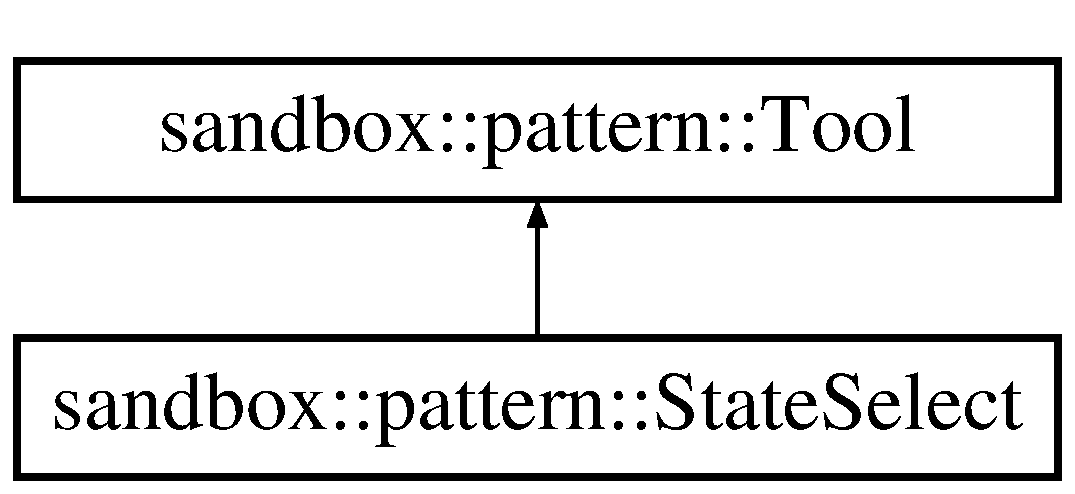
\includegraphics[height=2.000000cm]{classsandbox_1_1pattern_1_1_state_select}
\end{center}
\end{figure}
\subsection*{Public Member Functions}
\begin{DoxyCompactItemize}
\item 
void \hyperlink{classsandbox_1_1pattern_1_1_state_select_aaa4f406c5e76e77a34a0cf3a09c852a7}{on\-Mouse\-Down} (\hyperlink{classsandbox_1_1pattern_1_1_tool_controller}{Tool\-Controller} $\ast$controller)
\item 
void \hyperlink{classsandbox_1_1pattern_1_1_state_select_af8acb1db7b5a3400acf31aad1bde8768}{on\-Mouse\-Up} (\hyperlink{classsandbox_1_1pattern_1_1_tool_controller}{Tool\-Controller} $\ast$controller)
\item 
void \hyperlink{classsandbox_1_1pattern_1_1_state_select_a037ef0d19987035222019e006d08b4a4}{on\-Mouse\-Move} (\hyperlink{classsandbox_1_1pattern_1_1_tool_controller}{Tool\-Controller} $\ast$controller)
\end{DoxyCompactItemize}


\subsection{Member Function Documentation}
\hypertarget{classsandbox_1_1pattern_1_1_state_select_aaa4f406c5e76e77a34a0cf3a09c852a7}{\index{sandbox\-::pattern\-::\-State\-Select@{sandbox\-::pattern\-::\-State\-Select}!on\-Mouse\-Down@{on\-Mouse\-Down}}
\index{on\-Mouse\-Down@{on\-Mouse\-Down}!sandbox::pattern::StateSelect@{sandbox\-::pattern\-::\-State\-Select}}
\subsubsection[{on\-Mouse\-Down}]{\setlength{\rightskip}{0pt plus 5cm}void sandbox\-::pattern\-::\-State\-Select\-::on\-Mouse\-Down (
\begin{DoxyParamCaption}
\item[{{\bf Tool\-Controller} $\ast$}]{controller}
\end{DoxyParamCaption}
)\hspace{0.3cm}{\ttfamily [inline]}, {\ttfamily [virtual]}}}\label{classsandbox_1_1pattern_1_1_state_select_aaa4f406c5e76e77a34a0cf3a09c852a7}


Implements \hyperlink{classsandbox_1_1pattern_1_1_tool_a9878d4cea3771b76705f840134c980d8}{sandbox\-::pattern\-::\-Tool}.

\hypertarget{classsandbox_1_1pattern_1_1_state_select_a037ef0d19987035222019e006d08b4a4}{\index{sandbox\-::pattern\-::\-State\-Select@{sandbox\-::pattern\-::\-State\-Select}!on\-Mouse\-Move@{on\-Mouse\-Move}}
\index{on\-Mouse\-Move@{on\-Mouse\-Move}!sandbox::pattern::StateSelect@{sandbox\-::pattern\-::\-State\-Select}}
\subsubsection[{on\-Mouse\-Move}]{\setlength{\rightskip}{0pt plus 5cm}void sandbox\-::pattern\-::\-State\-Select\-::on\-Mouse\-Move (
\begin{DoxyParamCaption}
\item[{{\bf Tool\-Controller} $\ast$}]{controller}
\end{DoxyParamCaption}
)\hspace{0.3cm}{\ttfamily [inline]}, {\ttfamily [virtual]}}}\label{classsandbox_1_1pattern_1_1_state_select_a037ef0d19987035222019e006d08b4a4}


Implements \hyperlink{classsandbox_1_1pattern_1_1_tool_a4559b0a91622d26e3b531fd3dc9e42f6}{sandbox\-::pattern\-::\-Tool}.

\hypertarget{classsandbox_1_1pattern_1_1_state_select_af8acb1db7b5a3400acf31aad1bde8768}{\index{sandbox\-::pattern\-::\-State\-Select@{sandbox\-::pattern\-::\-State\-Select}!on\-Mouse\-Up@{on\-Mouse\-Up}}
\index{on\-Mouse\-Up@{on\-Mouse\-Up}!sandbox::pattern::StateSelect@{sandbox\-::pattern\-::\-State\-Select}}
\subsubsection[{on\-Mouse\-Up}]{\setlength{\rightskip}{0pt plus 5cm}void sandbox\-::pattern\-::\-State\-Select\-::on\-Mouse\-Up (
\begin{DoxyParamCaption}
\item[{{\bf Tool\-Controller} $\ast$}]{controller}
\end{DoxyParamCaption}
)\hspace{0.3cm}{\ttfamily [inline]}, {\ttfamily [virtual]}}}\label{classsandbox_1_1pattern_1_1_state_select_af8acb1db7b5a3400acf31aad1bde8768}


Implements \hyperlink{classsandbox_1_1pattern_1_1_tool_a3d82d69a33e32231d102e28eae555ca3}{sandbox\-::pattern\-::\-Tool}.



The documentation for this class was generated from the following file\-:\begin{DoxyCompactItemize}
\item 
F\-:/\-Projects/sandbox/src/pattern/\hyperlink{state_8h}{state.\-h}\end{DoxyCompactItemize}

\hypertarget{classsandbox_1_1_time_type}{\section{sandbox\-:\-:Time\-Type Class Reference}
\label{classsandbox_1_1_time_type}\index{sandbox\-::\-Time\-Type@{sandbox\-::\-Time\-Type}}
}


{\ttfamily \#include $<$timetype.\-h$>$}

\subsection*{Public Member Functions}
\begin{DoxyCompactItemize}
\item 
\hyperlink{classsandbox_1_1_time_type_ae6ad86008c1b53546e78b41f297395ad}{Time\-Type} (const int hour, const int minute)
\item 
double \hyperlink{classsandbox_1_1_time_type_adf071b75e3a518300e79b90de0dbe68b}{get\-Degree} () const 
\end{DoxyCompactItemize}


\subsection{Constructor \& Destructor Documentation}
\hypertarget{classsandbox_1_1_time_type_ae6ad86008c1b53546e78b41f297395ad}{\index{sandbox\-::\-Time\-Type@{sandbox\-::\-Time\-Type}!Time\-Type@{Time\-Type}}
\index{Time\-Type@{Time\-Type}!sandbox::TimeType@{sandbox\-::\-Time\-Type}}
\subsubsection[{Time\-Type}]{\setlength{\rightskip}{0pt plus 5cm}sandbox\-::\-Time\-Type\-::\-Time\-Type (
\begin{DoxyParamCaption}
\item[{const int}]{hour, }
\item[{const int}]{minute}
\end{DoxyParamCaption}
)}}\label{classsandbox_1_1_time_type_ae6ad86008c1b53546e78b41f297395ad}


\subsection{Member Function Documentation}
\hypertarget{classsandbox_1_1_time_type_adf071b75e3a518300e79b90de0dbe68b}{\index{sandbox\-::\-Time\-Type@{sandbox\-::\-Time\-Type}!get\-Degree@{get\-Degree}}
\index{get\-Degree@{get\-Degree}!sandbox::TimeType@{sandbox\-::\-Time\-Type}}
\subsubsection[{get\-Degree}]{\setlength{\rightskip}{0pt plus 5cm}double sandbox\-::\-Time\-Type\-::get\-Degree (
\begin{DoxyParamCaption}
{}
\end{DoxyParamCaption}
) const}}\label{classsandbox_1_1_time_type_adf071b75e3a518300e79b90de0dbe68b}


The documentation for this class was generated from the following files\-:\begin{DoxyCompactItemize}
\item 
F\-:/\-Projects/sandbox/src/\hyperlink{timetype_8h}{timetype.\-h}\item 
F\-:/\-Projects/sandbox/src/\hyperlink{timetype_8cpp}{timetype.\-cpp}\end{DoxyCompactItemize}

\hypertarget{classsandbox_1_1pattern_1_1_tool}{\section{sandbox\-:\-:pattern\-:\-:Tool Class Reference}
\label{classsandbox_1_1pattern_1_1_tool}\index{sandbox\-::pattern\-::\-Tool@{sandbox\-::pattern\-::\-Tool}}
}


{\ttfamily \#include $<$state.\-h$>$}

Inheritance diagram for sandbox\-:\-:pattern\-:\-:Tool\-:\begin{figure}[H]
\begin{center}
\leavevmode

\includegraphics[height=2.000000cm]{classsandbox_1_1pattern_1_1_tool}
\end{center}
\end{figure}
\subsection*{Public Member Functions}
\begin{DoxyCompactItemize}
\item 
virtual void \hyperlink{classsandbox_1_1pattern_1_1_tool_a9878d4cea3771b76705f840134c980d8}{on\-Mouse\-Down} (\hyperlink{classsandbox_1_1pattern_1_1_tool_controller}{Tool\-Controller} $\ast$)=0
\item 
virtual void \hyperlink{classsandbox_1_1pattern_1_1_tool_a3d82d69a33e32231d102e28eae555ca3}{on\-Mouse\-Up} (\hyperlink{classsandbox_1_1pattern_1_1_tool_controller}{Tool\-Controller} $\ast$)=0
\item 
virtual void \hyperlink{classsandbox_1_1pattern_1_1_tool_a4559b0a91622d26e3b531fd3dc9e42f6}{on\-Mouse\-Move} (\hyperlink{classsandbox_1_1pattern_1_1_tool_controller}{Tool\-Controller} $\ast$)=0
\end{DoxyCompactItemize}


\subsection{Member Function Documentation}
\hypertarget{classsandbox_1_1pattern_1_1_tool_a9878d4cea3771b76705f840134c980d8}{\index{sandbox\-::pattern\-::\-Tool@{sandbox\-::pattern\-::\-Tool}!on\-Mouse\-Down@{on\-Mouse\-Down}}
\index{on\-Mouse\-Down@{on\-Mouse\-Down}!sandbox::pattern::Tool@{sandbox\-::pattern\-::\-Tool}}
\subsubsection[{on\-Mouse\-Down}]{\setlength{\rightskip}{0pt plus 5cm}virtual void sandbox\-::pattern\-::\-Tool\-::on\-Mouse\-Down (
\begin{DoxyParamCaption}
\item[{{\bf Tool\-Controller} $\ast$}]{}
\end{DoxyParamCaption}
)\hspace{0.3cm}{\ttfamily [pure virtual]}}}\label{classsandbox_1_1pattern_1_1_tool_a9878d4cea3771b76705f840134c980d8}


Implemented in \hyperlink{classsandbox_1_1pattern_1_1_state_select_aaa4f406c5e76e77a34a0cf3a09c852a7}{sandbox\-::pattern\-::\-State\-Select}, and \hyperlink{classsandbox_1_1pattern_1_1_draw_tool_af43b828fa933c2ee66279f378cda067d}{sandbox\-::pattern\-::\-Draw\-Tool}.

\hypertarget{classsandbox_1_1pattern_1_1_tool_a4559b0a91622d26e3b531fd3dc9e42f6}{\index{sandbox\-::pattern\-::\-Tool@{sandbox\-::pattern\-::\-Tool}!on\-Mouse\-Move@{on\-Mouse\-Move}}
\index{on\-Mouse\-Move@{on\-Mouse\-Move}!sandbox::pattern::Tool@{sandbox\-::pattern\-::\-Tool}}
\subsubsection[{on\-Mouse\-Move}]{\setlength{\rightskip}{0pt plus 5cm}virtual void sandbox\-::pattern\-::\-Tool\-::on\-Mouse\-Move (
\begin{DoxyParamCaption}
\item[{{\bf Tool\-Controller} $\ast$}]{}
\end{DoxyParamCaption}
)\hspace{0.3cm}{\ttfamily [pure virtual]}}}\label{classsandbox_1_1pattern_1_1_tool_a4559b0a91622d26e3b531fd3dc9e42f6}


Implemented in \hyperlink{classsandbox_1_1pattern_1_1_state_select_a037ef0d19987035222019e006d08b4a4}{sandbox\-::pattern\-::\-State\-Select}, and \hyperlink{classsandbox_1_1pattern_1_1_draw_tool_a66e92b8b6ca5b9623203051bb31151bf}{sandbox\-::pattern\-::\-Draw\-Tool}.

\hypertarget{classsandbox_1_1pattern_1_1_tool_a3d82d69a33e32231d102e28eae555ca3}{\index{sandbox\-::pattern\-::\-Tool@{sandbox\-::pattern\-::\-Tool}!on\-Mouse\-Up@{on\-Mouse\-Up}}
\index{on\-Mouse\-Up@{on\-Mouse\-Up}!sandbox::pattern::Tool@{sandbox\-::pattern\-::\-Tool}}
\subsubsection[{on\-Mouse\-Up}]{\setlength{\rightskip}{0pt plus 5cm}virtual void sandbox\-::pattern\-::\-Tool\-::on\-Mouse\-Up (
\begin{DoxyParamCaption}
\item[{{\bf Tool\-Controller} $\ast$}]{}
\end{DoxyParamCaption}
)\hspace{0.3cm}{\ttfamily [pure virtual]}}}\label{classsandbox_1_1pattern_1_1_tool_a3d82d69a33e32231d102e28eae555ca3}


Implemented in \hyperlink{classsandbox_1_1pattern_1_1_state_select_af8acb1db7b5a3400acf31aad1bde8768}{sandbox\-::pattern\-::\-State\-Select}, and \hyperlink{classsandbox_1_1pattern_1_1_draw_tool_a3cb662ec466497fdfc9b69b2a4b1fcdb}{sandbox\-::pattern\-::\-Draw\-Tool}.



The documentation for this class was generated from the following file\-:\begin{DoxyCompactItemize}
\item 
F\-:/\-Projects/sandbox/src/pattern/\hyperlink{state_8h}{state.\-h}\end{DoxyCompactItemize}

\hypertarget{classsandbox_1_1pattern_1_1_tool_controller}{\section{sandbox\-:\-:pattern\-:\-:Tool\-Controller Class Reference}
\label{classsandbox_1_1pattern_1_1_tool_controller}\index{sandbox\-::pattern\-::\-Tool\-Controller@{sandbox\-::pattern\-::\-Tool\-Controller}}
}


{\ttfamily \#include $<$state.\-h$>$}

\subsection*{Public Member Functions}
\begin{DoxyCompactItemize}
\item 
void \hyperlink{classsandbox_1_1pattern_1_1_tool_controller_a7359815a0e7e9b1ad8c67de16e93332e}{on\-Mouse\-Down} ()
\item 
void \hyperlink{classsandbox_1_1pattern_1_1_tool_controller_ab49ae3a1fc34dd6f3ee342b23b80243e}{on\-Mouse\-Up} ()
\item 
void \hyperlink{classsandbox_1_1pattern_1_1_tool_controller_a44369d355a9baaf94e5a64f75b64dade}{on\-Mouse\-Move} ()
\end{DoxyCompactItemize}
\subsection*{Friends}
\begin{DoxyCompactItemize}
\item 
class \hyperlink{classsandbox_1_1pattern_1_1_tool_controller_a76e9adf1d0321729d4b28ce85a6825fd}{Tool}
\end{DoxyCompactItemize}


\subsection{Member Function Documentation}
\hypertarget{classsandbox_1_1pattern_1_1_tool_controller_a7359815a0e7e9b1ad8c67de16e93332e}{\index{sandbox\-::pattern\-::\-Tool\-Controller@{sandbox\-::pattern\-::\-Tool\-Controller}!on\-Mouse\-Down@{on\-Mouse\-Down}}
\index{on\-Mouse\-Down@{on\-Mouse\-Down}!sandbox::pattern::ToolController@{sandbox\-::pattern\-::\-Tool\-Controller}}
\subsubsection[{on\-Mouse\-Down}]{\setlength{\rightskip}{0pt plus 5cm}void sandbox\-::pattern\-::\-Tool\-Controller\-::on\-Mouse\-Down (
\begin{DoxyParamCaption}
{}
\end{DoxyParamCaption}
)\hspace{0.3cm}{\ttfamily [inline]}}}\label{classsandbox_1_1pattern_1_1_tool_controller_a7359815a0e7e9b1ad8c67de16e93332e}
\hypertarget{classsandbox_1_1pattern_1_1_tool_controller_a44369d355a9baaf94e5a64f75b64dade}{\index{sandbox\-::pattern\-::\-Tool\-Controller@{sandbox\-::pattern\-::\-Tool\-Controller}!on\-Mouse\-Move@{on\-Mouse\-Move}}
\index{on\-Mouse\-Move@{on\-Mouse\-Move}!sandbox::pattern::ToolController@{sandbox\-::pattern\-::\-Tool\-Controller}}
\subsubsection[{on\-Mouse\-Move}]{\setlength{\rightskip}{0pt plus 5cm}void sandbox\-::pattern\-::\-Tool\-Controller\-::on\-Mouse\-Move (
\begin{DoxyParamCaption}
{}
\end{DoxyParamCaption}
)\hspace{0.3cm}{\ttfamily [inline]}}}\label{classsandbox_1_1pattern_1_1_tool_controller_a44369d355a9baaf94e5a64f75b64dade}
\hypertarget{classsandbox_1_1pattern_1_1_tool_controller_ab49ae3a1fc34dd6f3ee342b23b80243e}{\index{sandbox\-::pattern\-::\-Tool\-Controller@{sandbox\-::pattern\-::\-Tool\-Controller}!on\-Mouse\-Up@{on\-Mouse\-Up}}
\index{on\-Mouse\-Up@{on\-Mouse\-Up}!sandbox::pattern::ToolController@{sandbox\-::pattern\-::\-Tool\-Controller}}
\subsubsection[{on\-Mouse\-Up}]{\setlength{\rightskip}{0pt plus 5cm}void sandbox\-::pattern\-::\-Tool\-Controller\-::on\-Mouse\-Up (
\begin{DoxyParamCaption}
{}
\end{DoxyParamCaption}
)\hspace{0.3cm}{\ttfamily [inline]}}}\label{classsandbox_1_1pattern_1_1_tool_controller_ab49ae3a1fc34dd6f3ee342b23b80243e}


\subsection{Friends And Related Function Documentation}
\hypertarget{classsandbox_1_1pattern_1_1_tool_controller_a76e9adf1d0321729d4b28ce85a6825fd}{\index{sandbox\-::pattern\-::\-Tool\-Controller@{sandbox\-::pattern\-::\-Tool\-Controller}!Tool@{Tool}}
\index{Tool@{Tool}!sandbox::pattern::ToolController@{sandbox\-::pattern\-::\-Tool\-Controller}}
\subsubsection[{Tool}]{\setlength{\rightskip}{0pt plus 5cm}friend class {\bf Tool}\hspace{0.3cm}{\ttfamily [friend]}}}\label{classsandbox_1_1pattern_1_1_tool_controller_a76e9adf1d0321729d4b28ce85a6825fd}


The documentation for this class was generated from the following file\-:\begin{DoxyCompactItemize}
\item 
F\-:/\-Projects/sandbox/src/pattern/\hyperlink{state_8h}{state.\-h}\end{DoxyCompactItemize}

\hypertarget{classsandbox_1_1_variant}{\section{sandbox\-:\-:Variant Class Reference}
\label{classsandbox_1_1_variant}\index{sandbox\-::\-Variant@{sandbox\-::\-Variant}}
}


{\ttfamily \#include $<$variant.\-h$>$}

\subsection*{Public Member Functions}
\begin{DoxyCompactItemize}
\item 
\hyperlink{classsandbox_1_1_variant_a0edc9e6694f15b9938dc40f68cc9464b}{Variant} ()
\item 
\hyperlink{classsandbox_1_1_variant_a762c4c281191a8bb303a317c0e0da8ef}{Variant} (double const value)
\item 
\hyperlink{classsandbox_1_1_variant_a965d4621a0d600a96d02cd696703e82c}{Variant} (float const value)
\item 
\hyperlink{classsandbox_1_1_variant_a8498e32ad2db5751c2b8111a9320a006}{Variant} (int const value)
\item 
\hyperlink{classsandbox_1_1_variant_a3a4600bcd2367d516888ea5ac45e5d25}{Variant} (char const $\ast$value)
\item 
\hyperlink{classsandbox_1_1_variant_a9699b3360dbd4cc4b12f6b5d59d80db0}{Variant} (std\-::string const \&value)
\item 
double \hyperlink{classsandbox_1_1_variant_adcf82c9304b1ab044afb5f511add9f9b}{to\-Double} () const 
\item 
float \hyperlink{classsandbox_1_1_variant_a49e80434a87f7ed714e386ca82e83160}{to\-Float} () const 
\item 
int \hyperlink{classsandbox_1_1_variant_a31944d8717dad852da7dd6927db7e5d6}{to\-Int} () const 
\item 
std\-::string \hyperlink{classsandbox_1_1_variant_a12c2380fc67baff5ac95c21ecf0b7304}{to\-String} () const 
\end{DoxyCompactItemize}
\subsection*{Friends}
\begin{DoxyCompactItemize}
\item 
std\-::ostream \& \hyperlink{classsandbox_1_1_variant_a586cf3576aee021c7b73c7871c6ce427}{operator$<$$<$} (std\-::ostream \&output, \hyperlink{classsandbox_1_1_variant}{Variant} const \&variant)
\end{DoxyCompactItemize}


\subsection{Detailed Description}
A union like type to store exactly one vale of the intrinsic or string types 

\subsection{Constructor \& Destructor Documentation}
\hypertarget{classsandbox_1_1_variant_a0edc9e6694f15b9938dc40f68cc9464b}{\index{sandbox\-::\-Variant@{sandbox\-::\-Variant}!Variant@{Variant}}
\index{Variant@{Variant}!sandbox::Variant@{sandbox\-::\-Variant}}
\subsubsection[{Variant}]{\setlength{\rightskip}{0pt plus 5cm}sandbox\-::\-Variant\-::\-Variant (
\begin{DoxyParamCaption}
{}
\end{DoxyParamCaption}
)}}\label{classsandbox_1_1_variant_a0edc9e6694f15b9938dc40f68cc9464b}
\hypertarget{classsandbox_1_1_variant_a762c4c281191a8bb303a317c0e0da8ef}{\index{sandbox\-::\-Variant@{sandbox\-::\-Variant}!Variant@{Variant}}
\index{Variant@{Variant}!sandbox::Variant@{sandbox\-::\-Variant}}
\subsubsection[{Variant}]{\setlength{\rightskip}{0pt plus 5cm}sandbox\-::\-Variant\-::\-Variant (
\begin{DoxyParamCaption}
\item[{double const}]{value}
\end{DoxyParamCaption}
)}}\label{classsandbox_1_1_variant_a762c4c281191a8bb303a317c0e0da8ef}
\hypertarget{classsandbox_1_1_variant_a965d4621a0d600a96d02cd696703e82c}{\index{sandbox\-::\-Variant@{sandbox\-::\-Variant}!Variant@{Variant}}
\index{Variant@{Variant}!sandbox::Variant@{sandbox\-::\-Variant}}
\subsubsection[{Variant}]{\setlength{\rightskip}{0pt plus 5cm}sandbox\-::\-Variant\-::\-Variant (
\begin{DoxyParamCaption}
\item[{float const}]{value}
\end{DoxyParamCaption}
)}}\label{classsandbox_1_1_variant_a965d4621a0d600a96d02cd696703e82c}
\hypertarget{classsandbox_1_1_variant_a8498e32ad2db5751c2b8111a9320a006}{\index{sandbox\-::\-Variant@{sandbox\-::\-Variant}!Variant@{Variant}}
\index{Variant@{Variant}!sandbox::Variant@{sandbox\-::\-Variant}}
\subsubsection[{Variant}]{\setlength{\rightskip}{0pt plus 5cm}sandbox\-::\-Variant\-::\-Variant (
\begin{DoxyParamCaption}
\item[{int const}]{value}
\end{DoxyParamCaption}
)}}\label{classsandbox_1_1_variant_a8498e32ad2db5751c2b8111a9320a006}
\hypertarget{classsandbox_1_1_variant_a3a4600bcd2367d516888ea5ac45e5d25}{\index{sandbox\-::\-Variant@{sandbox\-::\-Variant}!Variant@{Variant}}
\index{Variant@{Variant}!sandbox::Variant@{sandbox\-::\-Variant}}
\subsubsection[{Variant}]{\setlength{\rightskip}{0pt plus 5cm}sandbox\-::\-Variant\-::\-Variant (
\begin{DoxyParamCaption}
\item[{char const $\ast$}]{value}
\end{DoxyParamCaption}
)}}\label{classsandbox_1_1_variant_a3a4600bcd2367d516888ea5ac45e5d25}
\hypertarget{classsandbox_1_1_variant_a9699b3360dbd4cc4b12f6b5d59d80db0}{\index{sandbox\-::\-Variant@{sandbox\-::\-Variant}!Variant@{Variant}}
\index{Variant@{Variant}!sandbox::Variant@{sandbox\-::\-Variant}}
\subsubsection[{Variant}]{\setlength{\rightskip}{0pt plus 5cm}sandbox\-::\-Variant\-::\-Variant (
\begin{DoxyParamCaption}
\item[{std\-::string const \&}]{value}
\end{DoxyParamCaption}
)}}\label{classsandbox_1_1_variant_a9699b3360dbd4cc4b12f6b5d59d80db0}


\subsection{Member Function Documentation}
\hypertarget{classsandbox_1_1_variant_adcf82c9304b1ab044afb5f511add9f9b}{\index{sandbox\-::\-Variant@{sandbox\-::\-Variant}!to\-Double@{to\-Double}}
\index{to\-Double@{to\-Double}!sandbox::Variant@{sandbox\-::\-Variant}}
\subsubsection[{to\-Double}]{\setlength{\rightskip}{0pt plus 5cm}double sandbox\-::\-Variant\-::to\-Double (
\begin{DoxyParamCaption}
{}
\end{DoxyParamCaption}
) const\hspace{0.3cm}{\ttfamily [inline]}}}\label{classsandbox_1_1_variant_adcf82c9304b1ab044afb5f511add9f9b}
\hypertarget{classsandbox_1_1_variant_a49e80434a87f7ed714e386ca82e83160}{\index{sandbox\-::\-Variant@{sandbox\-::\-Variant}!to\-Float@{to\-Float}}
\index{to\-Float@{to\-Float}!sandbox::Variant@{sandbox\-::\-Variant}}
\subsubsection[{to\-Float}]{\setlength{\rightskip}{0pt plus 5cm}float sandbox\-::\-Variant\-::to\-Float (
\begin{DoxyParamCaption}
{}
\end{DoxyParamCaption}
) const\hspace{0.3cm}{\ttfamily [inline]}}}\label{classsandbox_1_1_variant_a49e80434a87f7ed714e386ca82e83160}
\hypertarget{classsandbox_1_1_variant_a31944d8717dad852da7dd6927db7e5d6}{\index{sandbox\-::\-Variant@{sandbox\-::\-Variant}!to\-Int@{to\-Int}}
\index{to\-Int@{to\-Int}!sandbox::Variant@{sandbox\-::\-Variant}}
\subsubsection[{to\-Int}]{\setlength{\rightskip}{0pt plus 5cm}int sandbox\-::\-Variant\-::to\-Int (
\begin{DoxyParamCaption}
{}
\end{DoxyParamCaption}
) const\hspace{0.3cm}{\ttfamily [inline]}}}\label{classsandbox_1_1_variant_a31944d8717dad852da7dd6927db7e5d6}
\hypertarget{classsandbox_1_1_variant_a12c2380fc67baff5ac95c21ecf0b7304}{\index{sandbox\-::\-Variant@{sandbox\-::\-Variant}!to\-String@{to\-String}}
\index{to\-String@{to\-String}!sandbox::Variant@{sandbox\-::\-Variant}}
\subsubsection[{to\-String}]{\setlength{\rightskip}{0pt plus 5cm}std\-::string sandbox\-::\-Variant\-::to\-String (
\begin{DoxyParamCaption}
{}
\end{DoxyParamCaption}
) const\hspace{0.3cm}{\ttfamily [inline]}}}\label{classsandbox_1_1_variant_a12c2380fc67baff5ac95c21ecf0b7304}


\subsection{Friends And Related Function Documentation}
\hypertarget{classsandbox_1_1_variant_a586cf3576aee021c7b73c7871c6ce427}{\index{sandbox\-::\-Variant@{sandbox\-::\-Variant}!operator$<$$<$@{operator$<$$<$}}
\index{operator$<$$<$@{operator$<$$<$}!sandbox::Variant@{sandbox\-::\-Variant}}
\subsubsection[{operator$<$$<$}]{\setlength{\rightskip}{0pt plus 5cm}std\-::ostream\& operator$<$$<$ (
\begin{DoxyParamCaption}
\item[{std\-::ostream \&}]{output, }
\item[{{\bf Variant} const \&}]{variant}
\end{DoxyParamCaption}
)\hspace{0.3cm}{\ttfamily [friend]}}}\label{classsandbox_1_1_variant_a586cf3576aee021c7b73c7871c6ce427}


The documentation for this class was generated from the following file\-:\begin{DoxyCompactItemize}
\item 
F\-:/\-Projects/sandbox/src/\hyperlink{variant_8h}{variant.\-h}\end{DoxyCompactItemize}

\chapter{File Documentation}
\hypertarget{chromaaberration_8cpp}{\section{F\-:/\-Projects/sandbox/src/boost/chromaaberration.cpp File Reference}
\label{chromaaberration_8cpp}\index{F\-:/\-Projects/sandbox/src/boost/chromaaberration.\-cpp@{F\-:/\-Projects/sandbox/src/boost/chromaaberration.\-cpp}}
}
{\ttfamily \#include \char`\"{}chromaaberration.\-h\char`\"{}}\\*
{\ttfamily \#include $<$boost/gil/extension/io/png\-\_\-io.\-hpp$>$}\\*
{\ttfamily \#include $<$boost/gil/image.\-hpp$>$}\\*
{\ttfamily \#include $<$boost/gil/image\-\_\-view.\-hpp$>$}\\*
{\ttfamily \#include $<$random$>$}\\*
{\ttfamily \#include $<$chrono$>$}\\*
{\ttfamily \#include $<$functional$>$}\\*
{\ttfamily \#include $<$vector$>$}\\*
{\ttfamily \#include $<$iostream$>$}\\*
\subsection*{Functions}
\begin{DoxyCompactItemize}
\item 
{\footnotesize template$<$typename Image\-View $>$ }\\void \hyperlink{chromaaberration_8cpp_ab87b6661141bbad34a893d5ae541378b}{color\-Aberration} (Image\-View source, Image\-View destination)
\item 
int \hyperlink{chromaaberration_8cpp_a3c04138a5bfe5d72780bb7e82a18e627}{main} (int argc, char $\ast$$\ast$argv)
\end{DoxyCompactItemize}


\subsection{Function Documentation}
\hypertarget{chromaaberration_8cpp_ab87b6661141bbad34a893d5ae541378b}{\index{chromaaberration.\-cpp@{chromaaberration.\-cpp}!color\-Aberration@{color\-Aberration}}
\index{color\-Aberration@{color\-Aberration}!chromaaberration.cpp@{chromaaberration.\-cpp}}
\subsubsection[{color\-Aberration}]{\setlength{\rightskip}{0pt plus 5cm}template$<$typename Image\-View $>$ void color\-Aberration (
\begin{DoxyParamCaption}
\item[{Image\-View}]{source, }
\item[{Image\-View}]{destination}
\end{DoxyParamCaption}
)\hspace{0.3cm}{\ttfamily [inline]}}}\label{chromaaberration_8cpp_ab87b6661141bbad34a893d5ae541378b}
\hypertarget{chromaaberration_8cpp_a3c04138a5bfe5d72780bb7e82a18e627}{\index{chromaaberration.\-cpp@{chromaaberration.\-cpp}!main@{main}}
\index{main@{main}!chromaaberration.cpp@{chromaaberration.\-cpp}}
\subsubsection[{main}]{\setlength{\rightskip}{0pt plus 5cm}int main (
\begin{DoxyParamCaption}
\item[{int}]{argc, }
\item[{char $\ast$$\ast$}]{argv}
\end{DoxyParamCaption}
)}}\label{chromaaberration_8cpp_a3c04138a5bfe5d72780bb7e82a18e627}

\hypertarget{chromaaberration_8h}{\section{F\-:/\-Projects/sandbox/src/boost/chromaaberration.h File Reference}
\label{chromaaberration_8h}\index{F\-:/\-Projects/sandbox/src/boost/chromaaberration.\-h@{F\-:/\-Projects/sandbox/src/boost/chromaaberration.\-h}}
}
\subsection*{Macros}
\begin{DoxyCompactItemize}
\item 
\#define \hyperlink{chromaaberration_8h_a82a90dbcb3c65be802dccb31f909bd02}{int\-\_\-p\-\_\-\-N\-U\-L\-L}~(int$\ast$)N\-U\-L\-L
\item 
\#define \hyperlink{chromaaberration_8h_acad208b3e5753b679e6ef8d761d53d9f}{png\-\_\-infopp\-\_\-\-N\-U\-L\-L}~(png\-\_\-infopp)N\-U\-L\-L
\end{DoxyCompactItemize}


\subsection{Macro Definition Documentation}
\hypertarget{chromaaberration_8h_a82a90dbcb3c65be802dccb31f909bd02}{\index{chromaaberration.\-h@{chromaaberration.\-h}!int\-\_\-p\-\_\-\-N\-U\-L\-L@{int\-\_\-p\-\_\-\-N\-U\-L\-L}}
\index{int\-\_\-p\-\_\-\-N\-U\-L\-L@{int\-\_\-p\-\_\-\-N\-U\-L\-L}!chromaaberration.h@{chromaaberration.\-h}}
\subsubsection[{int\-\_\-p\-\_\-\-N\-U\-L\-L}]{\setlength{\rightskip}{0pt plus 5cm}\#define int\-\_\-p\-\_\-\-N\-U\-L\-L~(int$\ast$)N\-U\-L\-L}}\label{chromaaberration_8h_a82a90dbcb3c65be802dccb31f909bd02}
\hypertarget{chromaaberration_8h_acad208b3e5753b679e6ef8d761d53d9f}{\index{chromaaberration.\-h@{chromaaberration.\-h}!png\-\_\-infopp\-\_\-\-N\-U\-L\-L@{png\-\_\-infopp\-\_\-\-N\-U\-L\-L}}
\index{png\-\_\-infopp\-\_\-\-N\-U\-L\-L@{png\-\_\-infopp\-\_\-\-N\-U\-L\-L}!chromaaberration.h@{chromaaberration.\-h}}
\subsubsection[{png\-\_\-infopp\-\_\-\-N\-U\-L\-L}]{\setlength{\rightskip}{0pt plus 5cm}\#define png\-\_\-infopp\-\_\-\-N\-U\-L\-L~(png\-\_\-infopp)N\-U\-L\-L}}\label{chromaaberration_8h_acad208b3e5753b679e6ef8d761d53d9f}

\hypertarget{main_8cpp}{\section{F\-:/\-Projects/sandbox/src/main.cpp File Reference}
\label{main_8cpp}\index{F\-:/\-Projects/sandbox/src/main.\-cpp@{F\-:/\-Projects/sandbox/src/main.\-cpp}}
}
{\ttfamily \#include $<$cstdlib$>$}\\*
{\ttfamily \#include $<$string$>$}\\*
{\ttfamily \#include $<$iostream$>$}\\*
{\ttfamily \#include $<$vector$>$}\\*
{\ttfamily \#include $<$random$>$}\\*
{\ttfamily \#include $<$chrono$>$}\\*
{\ttfamily \#include $<$functional$>$}\\*
{\ttfamily \#include $<$algorithm$>$}\\*
{\ttfamily \#include \char`\"{}shed.\-h\char`\"{}}\\*
{\ttfamily \#include \char`\"{}pattern/singleton.\-h\char`\"{}}\\*
{\ttfamily \#include \char`\"{}quicksort.\-h\char`\"{}}\\*
{\ttfamily \#include \char`\"{}options.\-h\char`\"{}}\\*
{\ttfamily \#include \char`\"{}variant.\-h\char`\"{}}\\*
\subsection*{Functions}
\begin{DoxyCompactItemize}
\item 
int \hyperlink{main_8cpp_a3c04138a5bfe5d72780bb7e82a18e627}{main} (int argc, char $\ast$$\ast$argv)
\end{DoxyCompactItemize}


\subsection{Function Documentation}
\hypertarget{main_8cpp_a3c04138a5bfe5d72780bb7e82a18e627}{\index{main.\-cpp@{main.\-cpp}!main@{main}}
\index{main@{main}!main.cpp@{main.\-cpp}}
\subsubsection[{main}]{\setlength{\rightskip}{0pt plus 5cm}int main (
\begin{DoxyParamCaption}
\item[{int}]{argc, }
\item[{char $\ast$$\ast$}]{argv}
\end{DoxyParamCaption}
)}}\label{main_8cpp_a3c04138a5bfe5d72780bb7e82a18e627}

\hypertarget{options_8h}{\section{F\-:/\-Projects/sandbox/src/options.h File Reference}
\label{options_8h}\index{F\-:/\-Projects/sandbox/src/options.\-h@{F\-:/\-Projects/sandbox/src/options.\-h}}
}
{\ttfamily \#include $<$map$>$}\\*
{\ttfamily \#include $<$string$>$}\\*
{\ttfamily \#include $<$ostream$>$}\\*
{\ttfamily \#include $<$istream$>$}\\*
{\ttfamily \#include $<$algorithm$>$}\\*
{\ttfamily \#include \char`\"{}variant.\-h\char`\"{}}\\*
\subsection*{Classes}
\begin{DoxyCompactItemize}
\item 
class \hyperlink{classsandbox_1_1_options}{sandbox\-::\-Options}
\end{DoxyCompactItemize}
\subsection*{Namespaces}
\begin{DoxyCompactItemize}
\item 
\hyperlink{namespacesandbox}{sandbox}
\end{DoxyCompactItemize}
\subsection*{Functions}
\begin{DoxyCompactItemize}
\item 
std\-::ostream \& \hyperlink{namespacesandbox_a8ca45cec79e562a7f2322662d281d1b4}{sandbox\-::operator$<$$<$} (std\-::ostream \&output, Options \&options)
\begin{DoxyCompactList}\small\item\em Writes all data to a output stream. \end{DoxyCompactList}\item 
std\-::istream \& \hyperlink{namespacesandbox_ab63c581d554f481ae6d06c434db5f7e5}{sandbox\-::operator$>$$>$} (std\-::istream \&input, Options \&options)
\begin{DoxyCompactList}\small\item\em Reads key value pairs from an input stream. it's throws Options\-::invalid\-\_\-format exception on misformatted input. \end{DoxyCompactList}\end{DoxyCompactItemize}

\hypertarget{singleton_8h}{\section{F\-:/\-Projects/sandbox/src/pattern/singleton.h File Reference}
\label{singleton_8h}\index{F\-:/\-Projects/sandbox/src/pattern/singleton.\-h@{F\-:/\-Projects/sandbox/src/pattern/singleton.\-h}}
}
\subsection*{Classes}
\begin{DoxyCompactItemize}
\item 
class \hyperlink{classsandbox_1_1pattern_1_1_singleton}{sandbox\-::pattern\-::\-Singleton}
\end{DoxyCompactItemize}
\subsection*{Namespaces}
\begin{DoxyCompactItemize}
\item 
\hyperlink{namespacesandbox}{sandbox}
\item 
\hyperlink{namespacesandbox_1_1pattern}{sandbox\-::pattern}
\end{DoxyCompactItemize}

\hypertarget{state_8h}{\section{F\-:/\-Projects/sandbox/src/pattern/state.h File Reference}
\label{state_8h}\index{F\-:/\-Projects/sandbox/src/pattern/state.\-h@{F\-:/\-Projects/sandbox/src/pattern/state.\-h}}
}
\subsection*{Classes}
\begin{DoxyCompactItemize}
\item 
class \hyperlink{classsandbox_1_1pattern_1_1_tool}{sandbox\-::pattern\-::\-Tool}
\item 
class \hyperlink{classsandbox_1_1pattern_1_1_draw_tool}{sandbox\-::pattern\-::\-Draw\-Tool}
\item 
class \hyperlink{classsandbox_1_1pattern_1_1_state_select}{sandbox\-::pattern\-::\-State\-Select}
\item 
class \hyperlink{classsandbox_1_1pattern_1_1_tool_controller}{sandbox\-::pattern\-::\-Tool\-Controller}
\end{DoxyCompactItemize}
\subsection*{Namespaces}
\begin{DoxyCompactItemize}
\item 
\hyperlink{namespacesandbox}{sandbox}
\item 
\hyperlink{namespacesandbox_1_1pattern}{sandbox\-::pattern}
\end{DoxyCompactItemize}

\hypertarget{strategy_8h}{\section{F\-:/\-Projects/sandbox/src/pattern/strategy.h File Reference}
\label{strategy_8h}\index{F\-:/\-Projects/sandbox/src/pattern/strategy.\-h@{F\-:/\-Projects/sandbox/src/pattern/strategy.\-h}}
}

\hypertarget{template_method_8h}{\section{F\-:/\-Projects/sandbox/src/pattern/template\-Method.h File Reference}
\label{template_method_8h}\index{F\-:/\-Projects/sandbox/src/pattern/template\-Method.\-h@{F\-:/\-Projects/sandbox/src/pattern/template\-Method.\-h}}
}
\subsection*{Classes}
\begin{DoxyCompactItemize}
\item 
class \hyperlink{class_abstract_algorithm}{Abstract\-Algorithm}
\item 
class \hyperlink{class_concrete_algorithm}{Concrete\-Algorithm}
\end{DoxyCompactItemize}

\hypertarget{quicksort_8h}{\section{F\-:/\-Projects/sandbox/src/quicksort.h File Reference}
\label{quicksort_8h}\index{F\-:/\-Projects/sandbox/src/quicksort.\-h@{F\-:/\-Projects/sandbox/src/quicksort.\-h}}
}
{\ttfamily \#include $<$vector$>$}\\*
{\ttfamily \#include $<$iterator$>$}\\*
{\ttfamily \#include \char`\"{}shed.\-h\char`\"{}}\\*
{\ttfamily \#include $<$iostream$>$}\\*
\subsection*{Namespaces}
\begin{DoxyCompactItemize}
\item 
\hyperlink{namespacesandbox}{sandbox}
\end{DoxyCompactItemize}
\subsection*{Functions}
\begin{DoxyCompactItemize}
\item 
{\footnotesize template$<$typename Iterator $>$ }\\void \hyperlink{namespacesandbox_a9f8d9538b5bfad2fd243b182598f994e}{sandbox\-::print\-Out} (Iterator front, Iterator back)
\item 
{\footnotesize template$<$typename Iterator $>$ }\\void \hyperlink{namespacesandbox_a7d82a406c267d30ff1f27c5ff300437a}{sandbox\-::quick\-Sort} (Iterator front, Iterator back)
\item 
{\footnotesize template$<$typename T $>$ }\\std\-::vector$<$ T $>$ \& \hyperlink{namespacesandbox_a85c255856530c2a1f629abb6bf2f4497}{sandbox\-::quick\-Sort} (std\-::vector$<$ T $>$ \&sortable)
\end{DoxyCompactItemize}

\hypertarget{shed_8h}{\section{F\-:/\-Projects/sandbox/src/shed.h File Reference}
\label{shed_8h}\index{F\-:/\-Projects/sandbox/src/shed.\-h@{F\-:/\-Projects/sandbox/src/shed.\-h}}
}
{\ttfamily \#include $<$string$>$}\\*
{\ttfamily \#include $<$algorithm$>$}\\*
{\ttfamily \#include $<$iterator$>$}\\*
{\ttfamily \#include $<$cstring$>$}\\*
\subsection*{Namespaces}
\begin{DoxyCompactItemize}
\item 
\hyperlink{namespacesandbox}{sandbox}
\end{DoxyCompactItemize}
\subsection*{Functions}
\begin{DoxyCompactItemize}
\item 
{\footnotesize template$<$typename Iterator $>$ }\\bool \hyperlink{namespacesandbox_a25a11dad06fc0cd1b3f9bc583f093636}{sandbox\-::is\-Palindrome} (Iterator front, Iterator back)
\item 
bool \hyperlink{namespacesandbox_a4a569da66e67b46889d0c0597b7196b0}{sandbox\-::is\-Palindrome} (std\-::string const \&str)
\item 
bool \hyperlink{namespacesandbox_a639859e1234594e142ea447fad2b3b34}{sandbox\-::is\-Palindrome} (char const $\ast$str)
\item 
bool \hyperlink{namespacesandbox_a563b930dc7888d8ab257fe747fa53487}{sandbox\-::is\-Little\-Endian} ()
\item 
bool \hyperlink{namespacesandbox_a550f00cb3d4e2ac434c7b76532e79573}{sandbox\-::is\-Big\-Endian} ()
\item 
{\footnotesize template$<$typename T $>$ }\\void \hyperlink{namespacesandbox_a78a289ddc885bdcb5383f1363c54db2c}{sandbox\-::swap} (T \&a, T \&b)
\item 
{\footnotesize template$<$typename Iterator $>$ }\\void \hyperlink{namespacesandbox_af7dc9a62c4e56b2b4c4a12ff6e82a237}{sandbox\-::swap\-In\-Range} (Iterator front, Iterator back)
\item 
std\-::string \& \hyperlink{namespacesandbox_acb1d210d07ad7665578cbcb47c995332}{sandbox\-::reverse} (std\-::string \&str)
\item 
char $\ast$ \hyperlink{namespacesandbox_a71d57df2b65e2db22f1b6126cf5305ec}{sandbox\-::reverse} (char $\ast$str)
\item 
std\-::string \& \hyperlink{namespacesandbox_aa4f703c0251f20815a2f7d99bf55b9a8}{sandbox\-::reverse\-Words} (std\-::string \&str)
\end{DoxyCompactItemize}

\hypertarget{timetype_8cpp}{\section{F\-:/\-Projects/sandbox/src/timetype.cpp File Reference}
\label{timetype_8cpp}\index{F\-:/\-Projects/sandbox/src/timetype.\-cpp@{F\-:/\-Projects/sandbox/src/timetype.\-cpp}}
}
{\ttfamily \#include \char`\"{}timetype.\-h\char`\"{}}\\*
{\ttfamily \#include $<$cmath$>$}\\*
{\ttfamily \#include $<$stdexcept$>$}\\*

\hypertarget{timetype_8h}{\section{F\-:/\-Projects/sandbox/src/timetype.h File Reference}
\label{timetype_8h}\index{F\-:/\-Projects/sandbox/src/timetype.\-h@{F\-:/\-Projects/sandbox/src/timetype.\-h}}
}
\subsection*{Classes}
\begin{DoxyCompactItemize}
\item 
class \hyperlink{classsandbox_1_1_time_type}{sandbox\-::\-Time\-Type}
\end{DoxyCompactItemize}
\subsection*{Namespaces}
\begin{DoxyCompactItemize}
\item 
\hyperlink{namespacesandbox}{sandbox}
\end{DoxyCompactItemize}

\hypertarget{variant_8h}{\section{F\-:/\-Projects/sandbox/src/variant.h File Reference}
\label{variant_8h}\index{F\-:/\-Projects/sandbox/src/variant.\-h@{F\-:/\-Projects/sandbox/src/variant.\-h}}
}
{\ttfamily \#include $<$string$>$}\\*
{\ttfamily \#include $<$ostream$>$}\\*
{\ttfamily \#include $<$istream$>$}\\*
\subsection*{Classes}
\begin{DoxyCompactItemize}
\item 
class \hyperlink{classsandbox_1_1_variant}{sandbox\-::\-Variant}
\end{DoxyCompactItemize}
\subsection*{Namespaces}
\begin{DoxyCompactItemize}
\item 
\hyperlink{namespacesandbox}{sandbox}
\end{DoxyCompactItemize}
\subsection*{Functions}
\begin{DoxyCompactItemize}
\item 
std\-::ostream \& \hyperlink{namespacesandbox_a1d6485022eb73d061719402a29c67183}{sandbox\-::operator$<$$<$} (std\-::ostream \&output, Variant const \&variant)
\end{DoxyCompactItemize}

%--- End generated contents ---

% Index
\newpage
\phantomsection
\addcontentsline{toc}{part}{Index}
\printindex

\end{document}
